\hypertarget{introduction}{%
	\section{Introduction}\label{introduction7}}

This chapter focuses on investigating the dynamic material response of epithelial domes to varying strain, tension, and pressure. In a morphogenetic context, pressure levels can vary significantly across a wide range of magnitudes and timescales in different situations \cite{torres-sanchez2021, choudhury2022a}. For example, during blastocyst development, luminal pressure doubles, leading to changes in cortical tension and cellular strain \cite{chan2019}.

In the case of epithelial domes, \citet{latorre2018} observed a broad spectrum of pressure levels throughout dome evolution, resulting in various cellular deformations and tissue behaviors including active-superelasticity. However, in this system, control is limited to the footprint of the domes, with no capability to control pressure and tension. To address this limitation, in this chapter, we will employ the monolayer inflator (MOLI) system to subject tissues to different strain and tension regimes and characterize the material response of epithelial tissues.

\hypertarget{measurement-of-dome-mechanics}{%
	\section{Measurement of dome mechanics}\label{measurement-of-dome-mechanics}}

To characterize the dynamics of the domes, we assumed that the shape of domes closely follows a spherical cap geometry, and hence we focused on the midsection (see Figure \ref{fig_7_1}). This  approximation is reasonable for domes with circular footprint. For spherical domes  supporting a membrane state of stress, mechanical equilibrium tangential to the surface implies that tension is isotropic and uniform tension, whereas mechanical equilibrium normal to the surface is expressed by Laplace's law \cite{latorre2018}. However, MOLI can also be applied to map the  heterogeneous and anisotropic tension of non-spherical domes, e.g.~resulting from non-circular footprints, applying curved Monolayer Stress Microscopy \cite{marin-llaurado2022}.

\begin{figure}
	\centering
	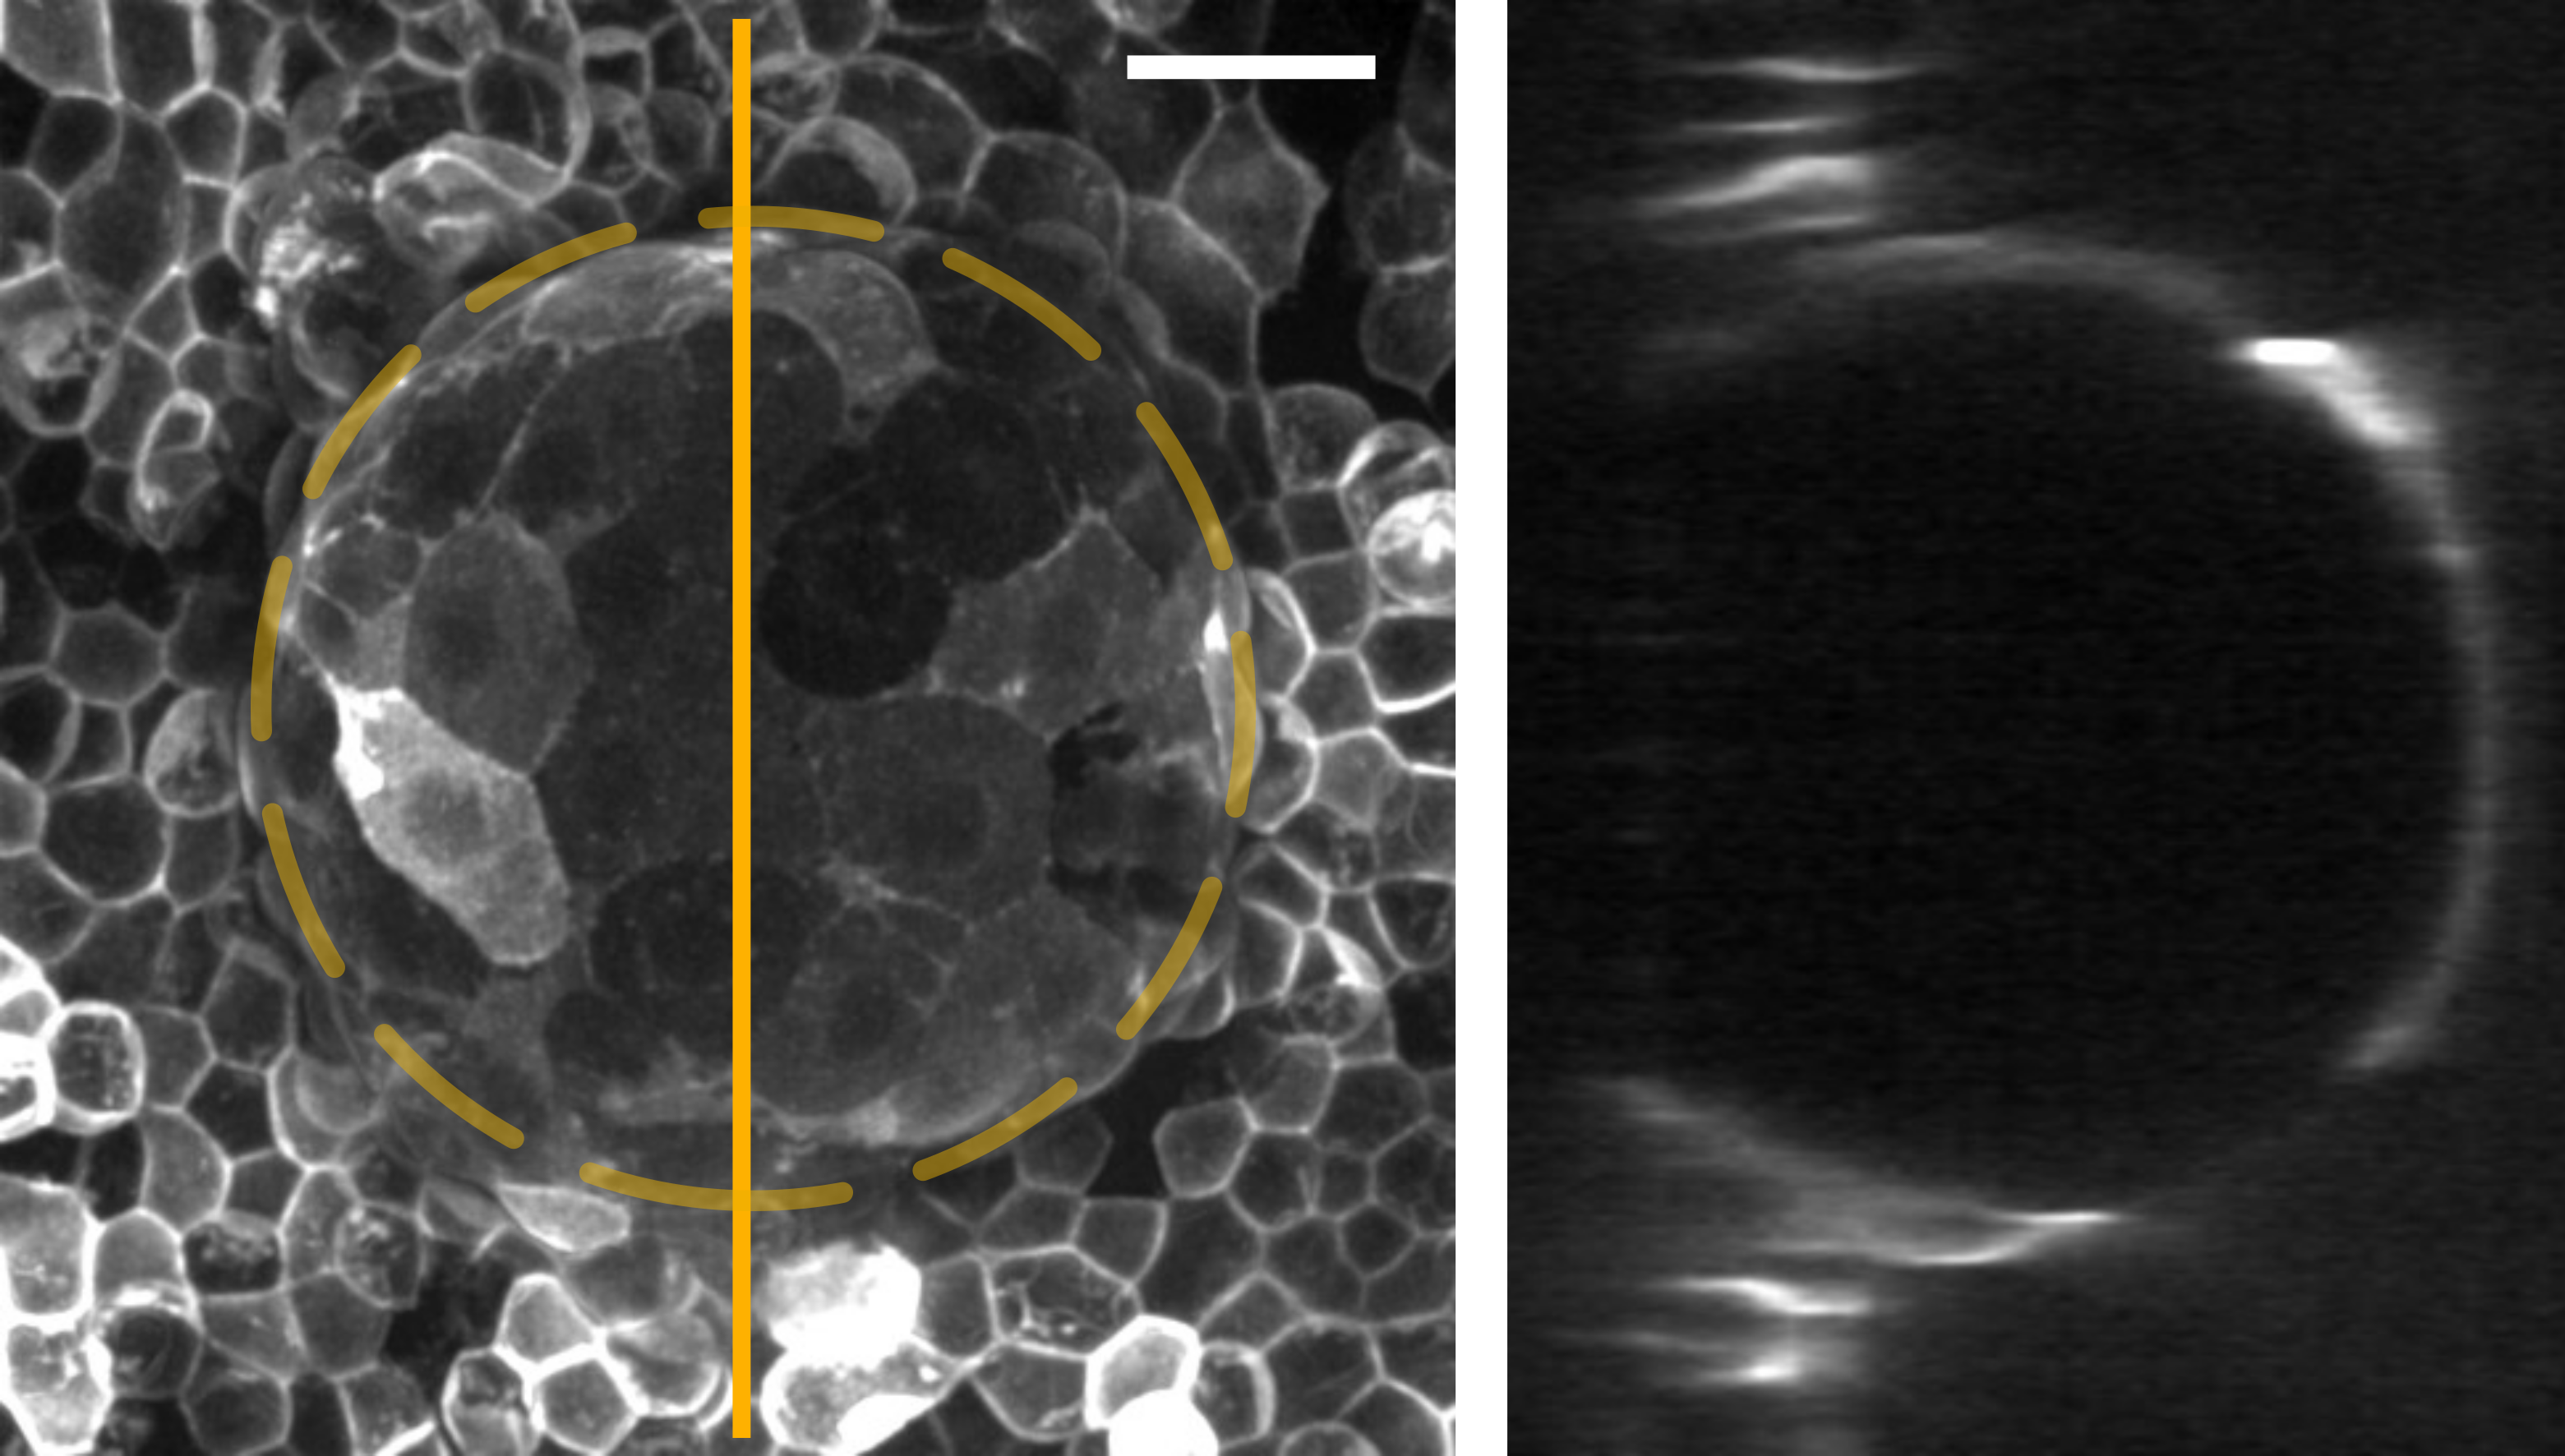
\includegraphics[width=0.8\textwidth]{chap7_realdome.png}
	\caption{\textbf{Epithelial dome generated by the MOLI device:} Maximum intensity projection of an MDCK dome (Left) . Dashed yellow line indicates the dome's footprint. Vertical yellow line crosses the center of the footprint, where the cross-section   (Right) shows the spherical shape of the dome. MDCK Cells were expressing CIBN CAAX GFP-488. Pressure, 200 Pa. Scale bar is $20 \mu m$.
	} \label{fig_7_1}
\end{figure}

From the cross-section, we measured the height $h$ and base radius $a$ of each dome, which allowed us to calculate the radius of curvature $R$ as
\begin{equation}
	\label{eqn:radiuscurve}
	R = \frac{h^2 + a^2}{2h}.
\end{equation}
Additionally, MOLI provides a direct readout of pressure $\Delta P$, allowing us to compute the tension ($\sigma$) using Laplace's law
\begin{equation}
	\label{eqn:laplace}
	\sigma = \frac{\Delta PR }{2} .
\end{equation}

To quantify dome deformation, we used the areal strain measure, which is defined as the difference between the dome surface area ($A$) and the area of the footprint ($A_{0}$) normalized by the latter, leading to
\begin{equation}
	\label{eqn:arealstrain}
	\epsilon = \frac{A - A_{0}}{A_{0}} = \frac{\pi(h^2 + a^2) - \pi a^2}{\pi a^2} = \frac{h^2}{a^2} .
\end{equation}
To obtain the temporal evolution of the dome’s geometry, we generated kymographs of the top section of the domes. These kymographs provide the time evolution of $h$. Given $a$ and the applied pressure as a function of time, we computed tensions and strain using the relations above.

\hypertarget{epithelial-domes-at-constant-pressure}{%
	\section{Epithelial domes at constant
		pressure}\label{epithelial-domes-at-constant-pressure}}

First, we systematically applied varying pressures ranging from 0-400 \unit{\pascal} to the domes. However, we observed that domes could not form at pressures lower than 50-100 \unit{\pascal} due to cell-substrate adhesion forces. Conversely, high pressures resulted in tissue delamination beyond the boundary of the patterned footprint. We determined that 200 \unit{\pascal} allowed the domes to form without delamination, falling within the previously reported pressure range \cite{choudhury2022,marin-llaurado2022}.

\begin{figure}[b!]
	\centering
	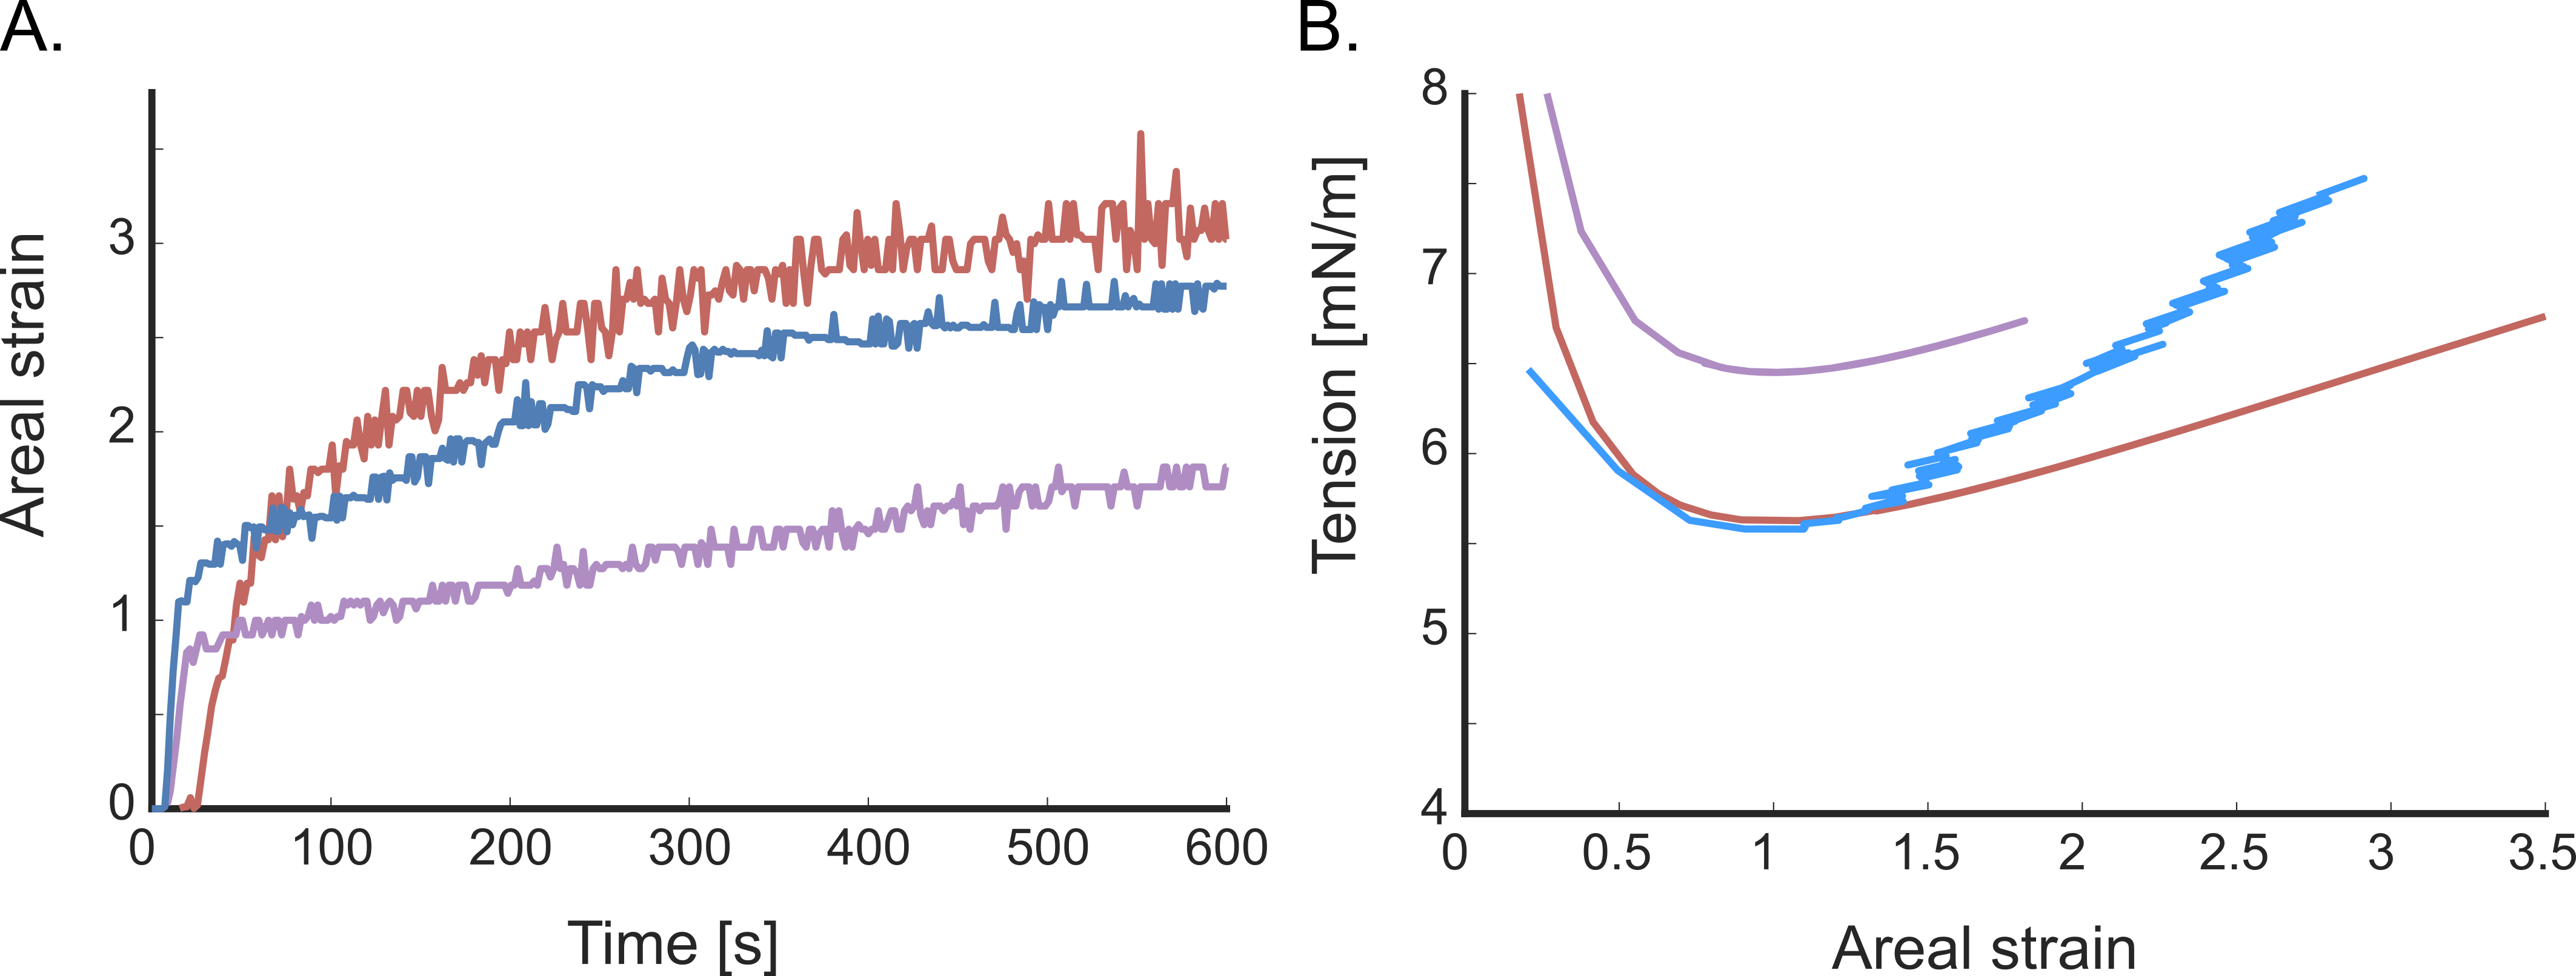
\includegraphics[width=\textwidth]{chap7_constpressure.png}
	\caption{\label{fig_7_3} \textbf{Epithelial domes at constant pressure}: Dynamic response of three representative domes at a constant pressure of 200 Pa (Domes with base radius: red 56 $\mu m$, blue 63 $\mu m$, purple 42 $\mu m$): (A) Areal strain increases and reaches a steady state at around 5 minutes, and we can clearly see variability in the maximum strains. (B) The same domes produce a peculiar tension and strain curve. In an inset on top, all three curves collapse onto a single  master curve, when tension $\sigma$ is normalized by base radius $a$ and plotted with respect to areal strain $\epsilon$. (representative of 12 domes)
	}
\end{figure}

When domes were subjected to a constant pressure of 200 \unit{\pascal}, they underwent a significant increase in areal strain during the first three to five minutes of pressure application. Following this initial increase, the areal strain reached a plateau and remained relatively constant for the next 5-10 minutes (see Figure \ref{fig_7_3} A). Notably, our measurements also indicated considerable variability in the maximum strain achieved by domes for the same pressure, with strains ranging from 50\% to 300\%. Nevertheless, the stabilization in strain across all the domes suggested that the epithelial tissue reached a mechanical steady state.

We then plotted the tension-strain relationship of these domes, systematically finding a non-monotonic curve similar to the Nike "swoosh" symbol (see Figure \ref{fig_7_3} B). At low strains, the tension within the domes is very high, followed by a decline to a minimum value at an areal strain of 100\%, where the dome adopts a hemispherical shape. Tension then increases  again, but the rate of increase is slower than the rate at which tension decreases at lower strains. This non-monotonic tension-strain curve is at odds with previous measurements of tension-strain relations in spontaneously fluctuating domes \cite{latorre2018,marin-llaurado2022} or in cell monolayers subjected to uniaxial stretch \cite{duque2023}. The fact that strains and tensions strongly varied from dome to dome but the minimum of tension was achieved precisely at 100\% areal strain for all domes suggested that this behavior is related to the nature of our measurement. 

Our measurement of the stress-strain relation only uses (1) mechanical equilibrium, encoded by Laplace's law, and (2) the geometrical relations between the radius of curvature $R$ of the dome, the footprint radius $a$, the height $h$ and the areal strain $\epsilon$. The geometric Eqs.~(\ref{eqn:radiuscurve},\ref{eqn:arealstrain}) can be combined to find an explicit relation between radius of curvature and strain
\begin{equation}
	R = \frac{h^2/a^2 + 1}{2h/a^2} = a\frac{\epsilon + 1}{\sqrt{\epsilon}},
\end{equation}
which when plugged into Laplace's law in Eq.~(\ref{eqn:laplace}) results in 
\begin{equation}
	\label{eqn:isobaric}
	\frac{\sigma}{a \Delta P} = \frac{1}{4}  \frac{\epsilon + 1}{\sqrt{\epsilon}}.
\end{equation}
This relation relates two non-dimensional quantities. Since in the experiments reported in Figure \ref{fig_7_3} pressure $\Delta P$ and footprint radius $a$ are constant, this relation shows that tension should be proportional to $(\epsilon + 1)/\sqrt{\epsilon}$ irrespective of the mechanical response of the tissue, as a result of geometry and mechanical equilibrium. For small strains ($\epsilon\ll 1$), we have $\sigma \propto 1/\sqrt{\epsilon}$, whereas for large strains $\epsilon\gg 1$, we have $\sigma \propto \sqrt{\epsilon}$ in agreement with the non-monotonic measured stress-strain curves. A geometric interpretation of the isobaric curve is shown in Figure \ref{fig_7_4}, which reflects the fact that the radius of curvature of a spherical dome of fixed footprint is minimum when the dome is half sphere. When represented according to Eq.~(\ref{eqn:isobaric}), all tension-strain curves collapse to a master curve reflecting the hypotheses of the measurement (see Fig. \ref{fig_7_3} B inset).

\begin{figure}
	\centering
	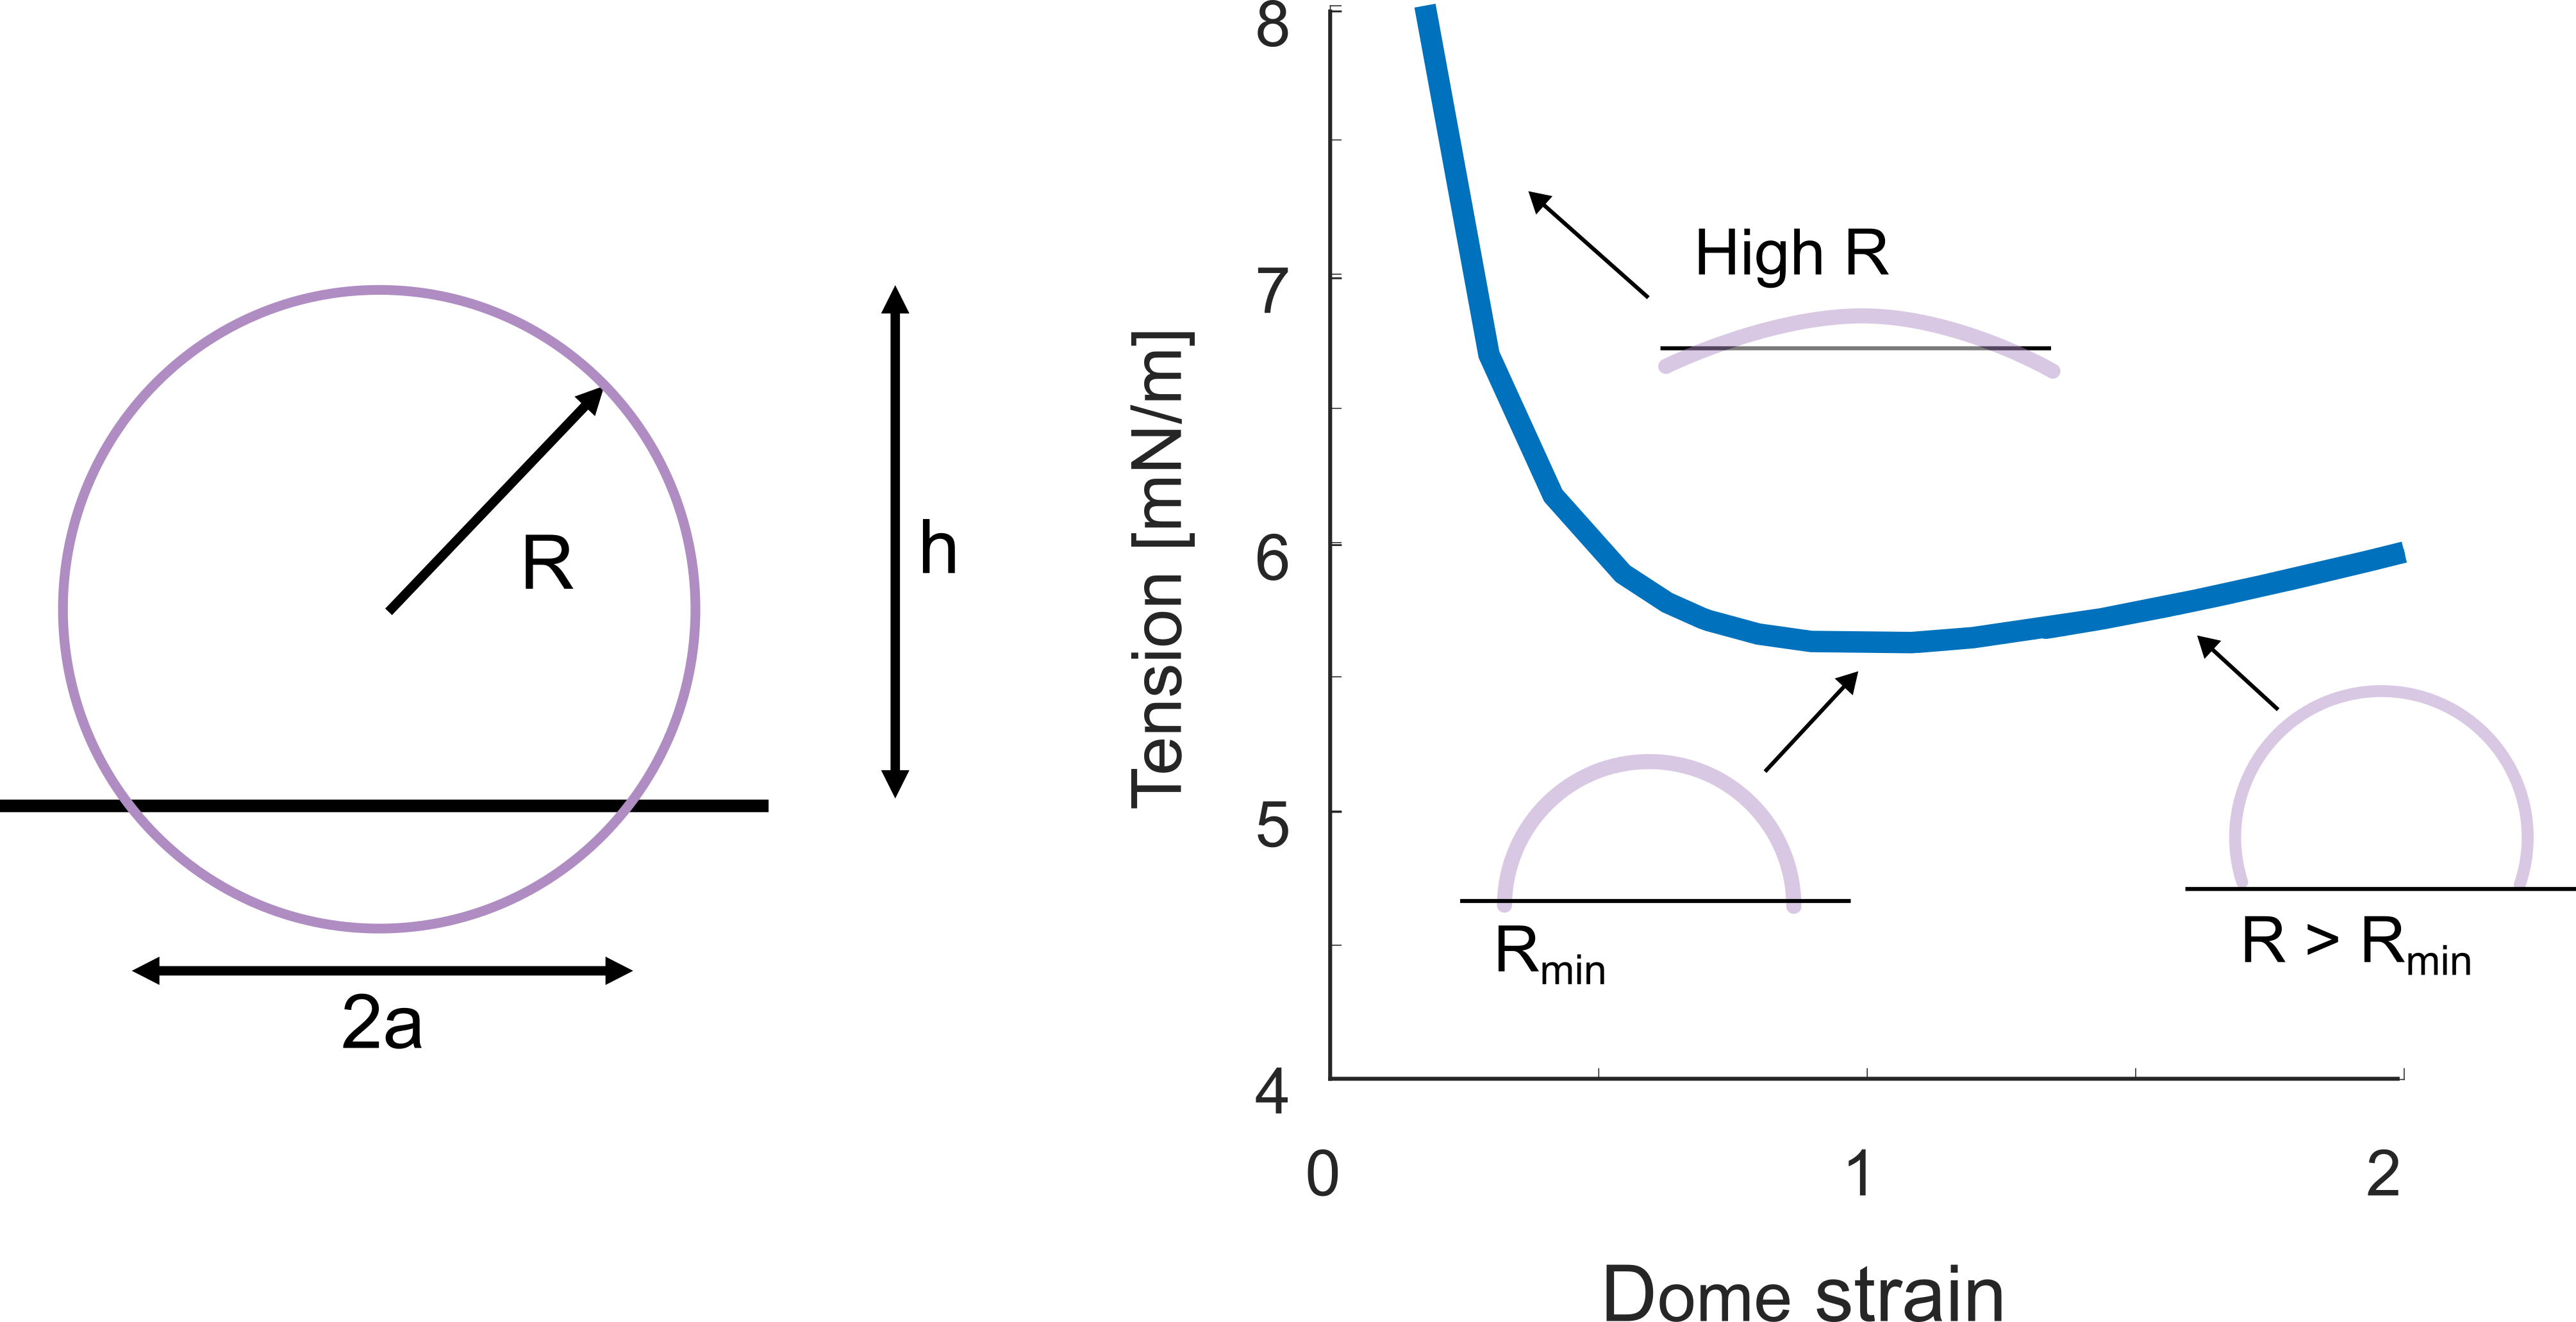
\includegraphics[width=0.8\textwidth]{chap7_radius.png}
	\caption{\label{fig_7_4} \textbf{Illustrative explanation for isobaric curve}: Tension and strain are related to each other through the geometric constraint of a spherical cap. Here, the base radius (a) is constant, so the radius of curvature is almost infinite for domes with very small strains (<0.05). As the strain increases, the radius of curvature decreases to a minimum corresponding to the base radius. Then it continues to increase again.	
	}
\end{figure}

%The tension-strain relationship of the domes can be explained by the geometric constraints imposed by the dome system and force balance. Laplace’s law implies that for a constant pressure, the tension within the dome is directly proportional to its radius of curvature. Domes with low strain are close to being flat monolayers and have a high value of the radius of curvature, which leads to a correspondingly high tension  (see Figure \ref{fig_7_4}). As the dome inflates, the radius of curvature subsequently diminishes to a minimum upon adopting a hemispherical shape. Since the dome always maintains a spherical shape, the radius of curvature, areal strain, and tension are all interconnected. The curve's expression can be derived by substituting areal strain ($\epsilon$) in the expression of radius of curvature ($R$) (Equation \ref{eqn:radiuscurve})


The previous discussion shows that Eq.~(\ref{eqn:isobaric}) alone does not say anything about the mechanical response of the epithelial monolayer. It just characterizes the locus of tension-strain states of a spherical dome that respects the physical constraint of mechanical equilibrium. This relation also shows the non-trivial relation between the pressure-controlled mechanical ensemble of MOLI, very natural for pressurized lumens, and more common tension-controlled  or strain-controlled ensembles.
%\marino{[This would be eloquently illustrated by showing tension vs time, but probably not needed]} Nimesh's Reply: LATER. 
Hence, the dynamics of Figure \ref{fig_7_3} A cannot be interpreted as neither stress-relaxation nor creep experiments. This figure also shows that during their trajectory along the isobaric curve, the tissue experiences a time-dependent relaxation towards a steady-state strain, and hence to a steady-state tension according to the isobaric relation Eq.~(\ref{eqn:isobaric}). Using a mechanical analogy, we can interpret that during these dynamics out-of-equilibrium (viscous) stresses relax and we are left with a pair $(\epsilon^*, \sigma^*)_{\Delta P}$ along a steady-state constitutive relation $\sigma^{\rm ss}(\epsilon)$ of the tissue. In the next section, we discuss how to use this principle to measure this constitutive relation.


%These measurements imply that when a step pressure is applied, the inflating dome undergoes a non-steady-state with out-of-equilibrium stresses while experiencing high tension related to high radius of curvature. The dome then rapidly inflates by following the tension-strain curve dictated by equation \ref{eqn:isobaric} to achieve a steady state. In this steady state, the external pressure is balanced with equilibrium tissue tension. It is evident that this tension-strain curve observed does not represent the quasi-static material response of the epithelial tissue. To determine the true tension strain relation, a different experimental strategy will be adopted in the following section.



\hypertarget{constitutive-relation-of-epithelia}{%
	\section{Steady-state constitutive relation of
		epithelia}\label{constitutive-relation-of-epithelia}}

Viewing the cell monolayer as a material sheet, we sought to characterize the stress-strain relation $\sigma^{\rm ss}(\epsilon)$ under quasi-static or steady-state conditions using MOLI \cite{latorre2018,duque2023}. If such a relation were to exist, they it should intersect the family of isobaric curves as we sweep $\Delta P$, see Fig. \ref{fig_7_5} A, and hence, in principle, we should be able to track it by identifying steady state pairs  $(\epsilon^*, \sigma^*)_{\Delta P}$ at different pressures.

\begin{figure}[h!]
	\centering
	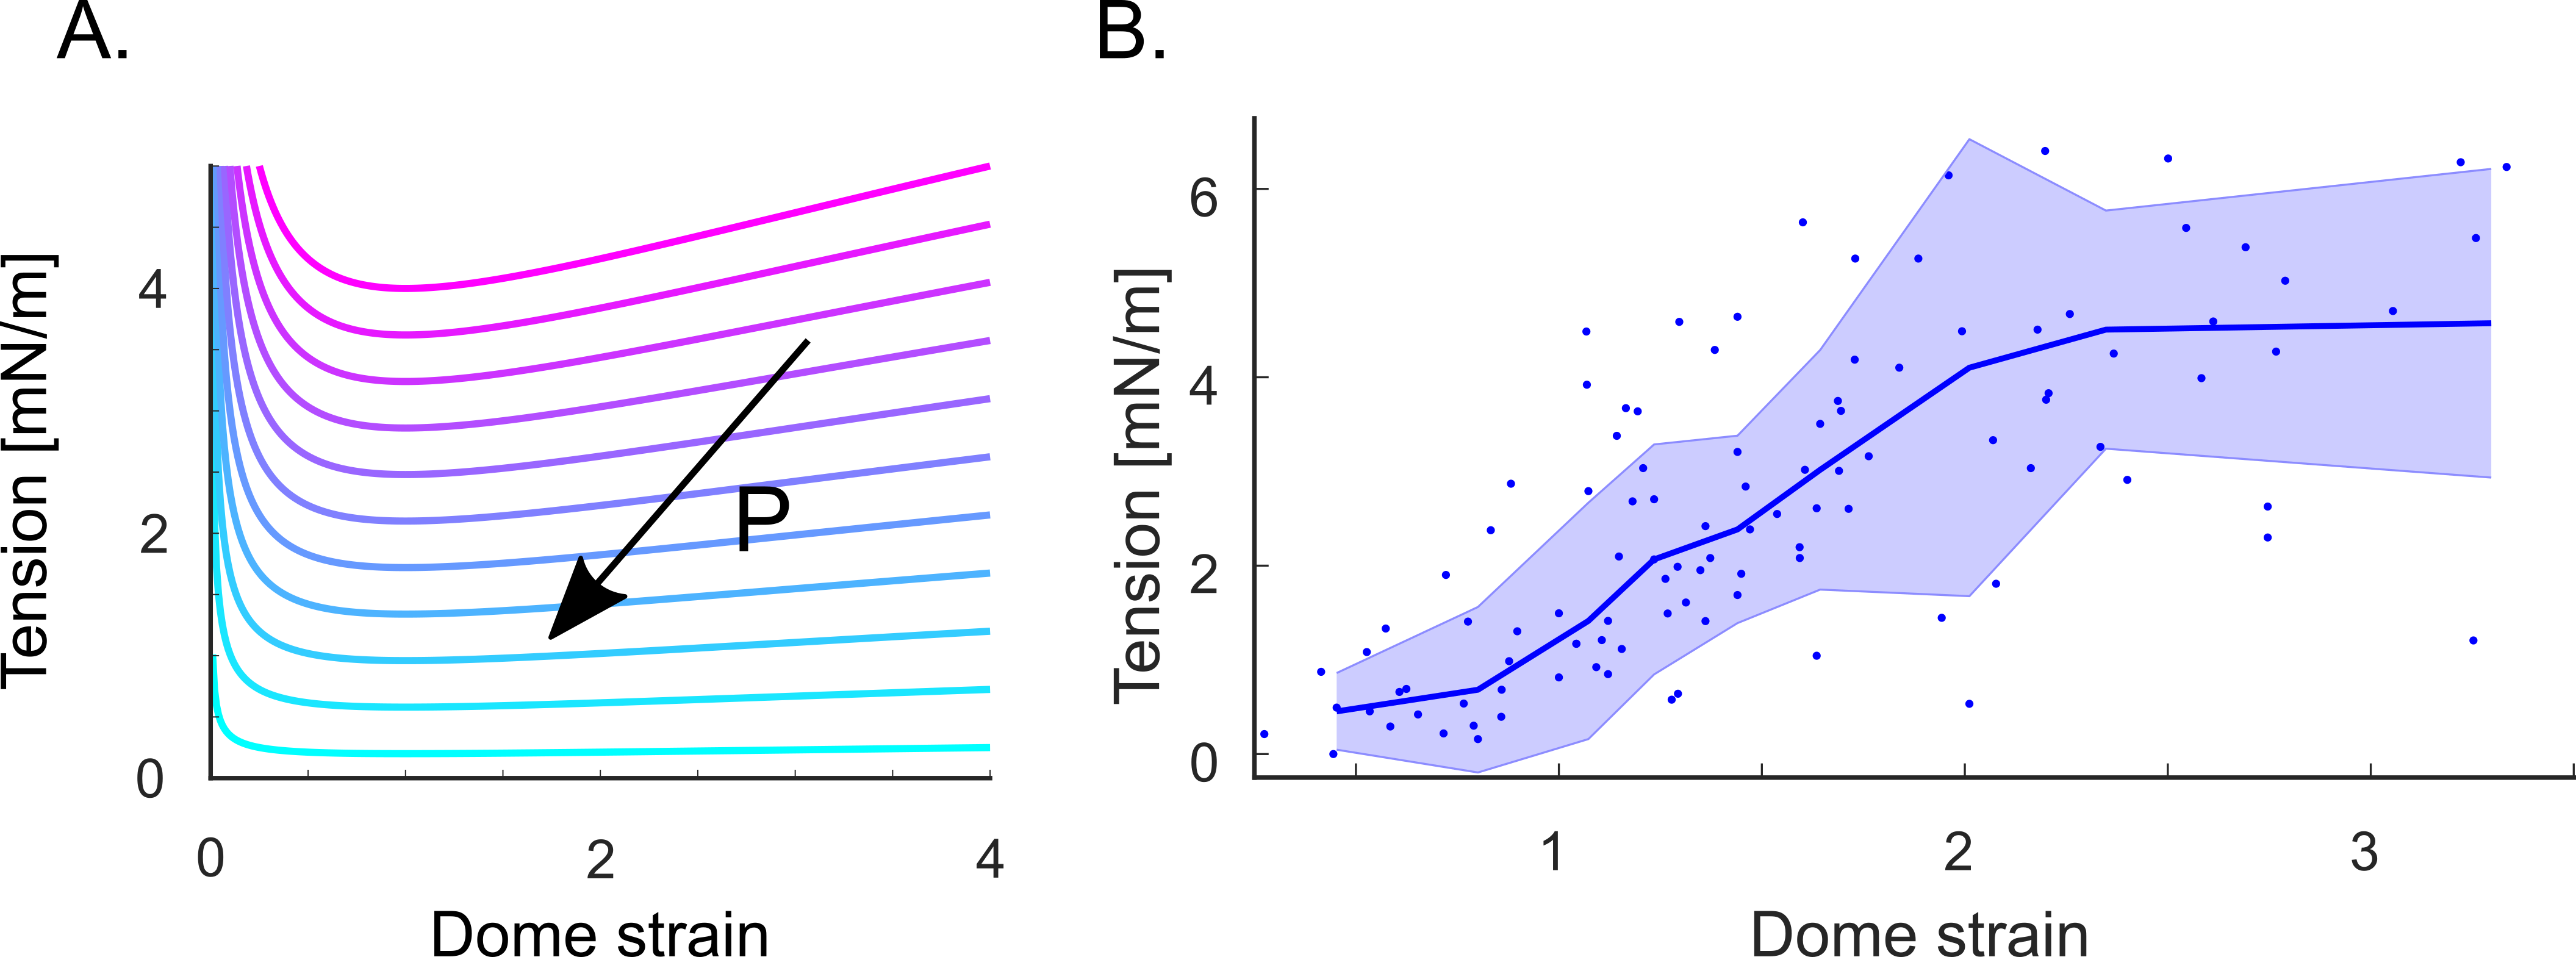
\includegraphics[width=\textwidth]{chap7_constitutivelaw.png}
	\caption{\label{fig_7_5}
		% \marino{[For paper, I would plot the two graphs above with the same ranges of tension/strain and with the same aspect ratio. I would also indicate the numerical value of $\Delta P$ for selected curves (or as a colorbar), and then the arrow with P is not needed, for a representative $a$, and would sketch a putative relation $\sigma^{\rm ss}(\epsilon)$ in A. In B, I assume you consider domes with different $a$, is that right?]} Nimesh's reply: AGREE, I WILL PREPARE IT FOR THE PAPER, Yes we have different size of domes in the dataset
		\textbf{Steady-state constitutive Relation of epithelial monolayers}: (A) We set up experiments to probe the steady state at different pressures. We will start from the highest pressure, move along the isobaric line and achieve a steady state, and then move down to the next curve, and so on.	(B) The constitutive relation between dome strain and tissue tension was experimentally obtained (n=12). The line and shaded area represent the median and standard deviation, respectively, by binning 13 points in each bin.}
\end{figure}

To implement this approach, progressively increasing pressure to track steady states is not feasible due to the existence of a pressure threshold for delamination. Instead, we swept pressures by deflating domes in steps. Specifically, we applied a pressure of 200 \unit{\pascal} for 5 minutes, allowing the dome to reach a steady state. We then reduced the pressure in increments of 20 \unit{\pascal}, allowing the dome to reach steady state at each step. This process continued until the dome was completely deflated. This approach allowed us to collect steady state tension-strain pairs that should lie on the curve $\sigma^{\rm ss}(\epsilon)$, hence mapping the steady-state constitutive relation of the tissue, Fig. \ref{fig_7_5} B. The resulting constitutive relation showed an initial increase in tension with strain for lower strains. For larger strains, the tension plateaued, consistent with earlier studies on MDCK domes. It is important to note the significant variability in dome-to-dome tension, with recorded tensions around 4.5 \unit{mN/m} with the same order of magnitude as those in previous studies \cite{latorre2018,marin-llaurado2022}. In summary, we show that MOLI can be used to map the steady-state constitutive relation of a tissue by stepwise pressure reduction. We probe next the dynamical material response.

\hypertarget{dynamics-of-the-epithelia-domes}{\section{Dynamics of the epithelial domes}\label{dynamics-of-the-epithelial-domes}}

Next, we investigated the dynamic material response of the domes by conducting cyclic pressurization experiments. We subjected the domes to a triangular wave of pressure with a magnitude of 200 Pa at three distinct timescales, as depicted in Figure~\ref{fig_7_6}. The selected timescales of 20s, 266s, and 2000s were based on existing literature on tissue remodeling, particularly the work of \citet{khalilgharibi2019} and \citet{casares2015}. These studies demonstrated that stress relaxation in tissues occurs from tens of seconds to minute timescales due to F-actin remodeling and myosin-driven contractility. Even faster deformation rates, which have been studied using different methods \cite{khalilgharibi2019}, are not accessible to the current implementation of MOLI because of the microscope’s imaging speed.
% Additionally, in some cases, even faster deformation at timescales of a few seconds has been shown to impact cell remodeling \cite{andreu2021a} 
%\marino{[I don't understand this sentence. Impact how? I am not sure this paper is so relevant here. Charras' studies have shown a power-law rheology of tissues at very short time-scales. Maybe, you could say, or not ``Faster deformation rates, which have been studied using different methods \cite{khalilgharibi2019}, are not accessible to the current implementation of MOLI because of the microscope’s imaging speed'']}. Nimesh's reply: I AGREE
%In our device, the fastest cycle that could be probed was limited to 20s because of the microscope’s imaging speed.
\begin{center}
	\begin{table}[h!]
		\label{tab:hysteresis}
		\centering
		\begin{tabular}{c c c c}
			& Fast & Moderate & Slow \\ 
			Time period (s) & 20   & 266      & 2000 \\ 
			Rates (Pa/s)    & 20   & 1.5      & 0.2  \\ 
		\end{tabular}
		\caption{Pressure rates used for cyclic stretching experiments}
	\end{table}
\end{center}
\vspace{-2em}

For the fastest cycles, we observed that the maximum strain achieved by the domes in each cycle increased until they reached a steady state oscillation around 600 seconds.
%\marino{around 600 seconds ?? [ by the end of the experiment]}. Nimesh's reply: YES
The experiment was conducted over 1200 seconds, equivalent to 60 cycles, during which we observed a cumulative buildup of strain over time. In the loading phase, the domes underwent stretching, while during the unloading phase, they experienced unstretching but failed to revert to zero strain after the initial cycles. In the concluding cycles, we noted that the dome oscillated between two distinct states of strain, resembling a limit cycle (see Fig. \ref{fig_7_6} B top).

A similar response was observed for the moderate cycles, where the domes were stretched for five cycles of 266s each. Strain accumulated in the first two cycles, with strains reaching higher values than those observed in the fast case (see Fig.~\ref{fig_7_6} B middle). After the third cycle, the dome appeared to reach a stable limit cycle.

\begin{figure}[h!]
	\centering
	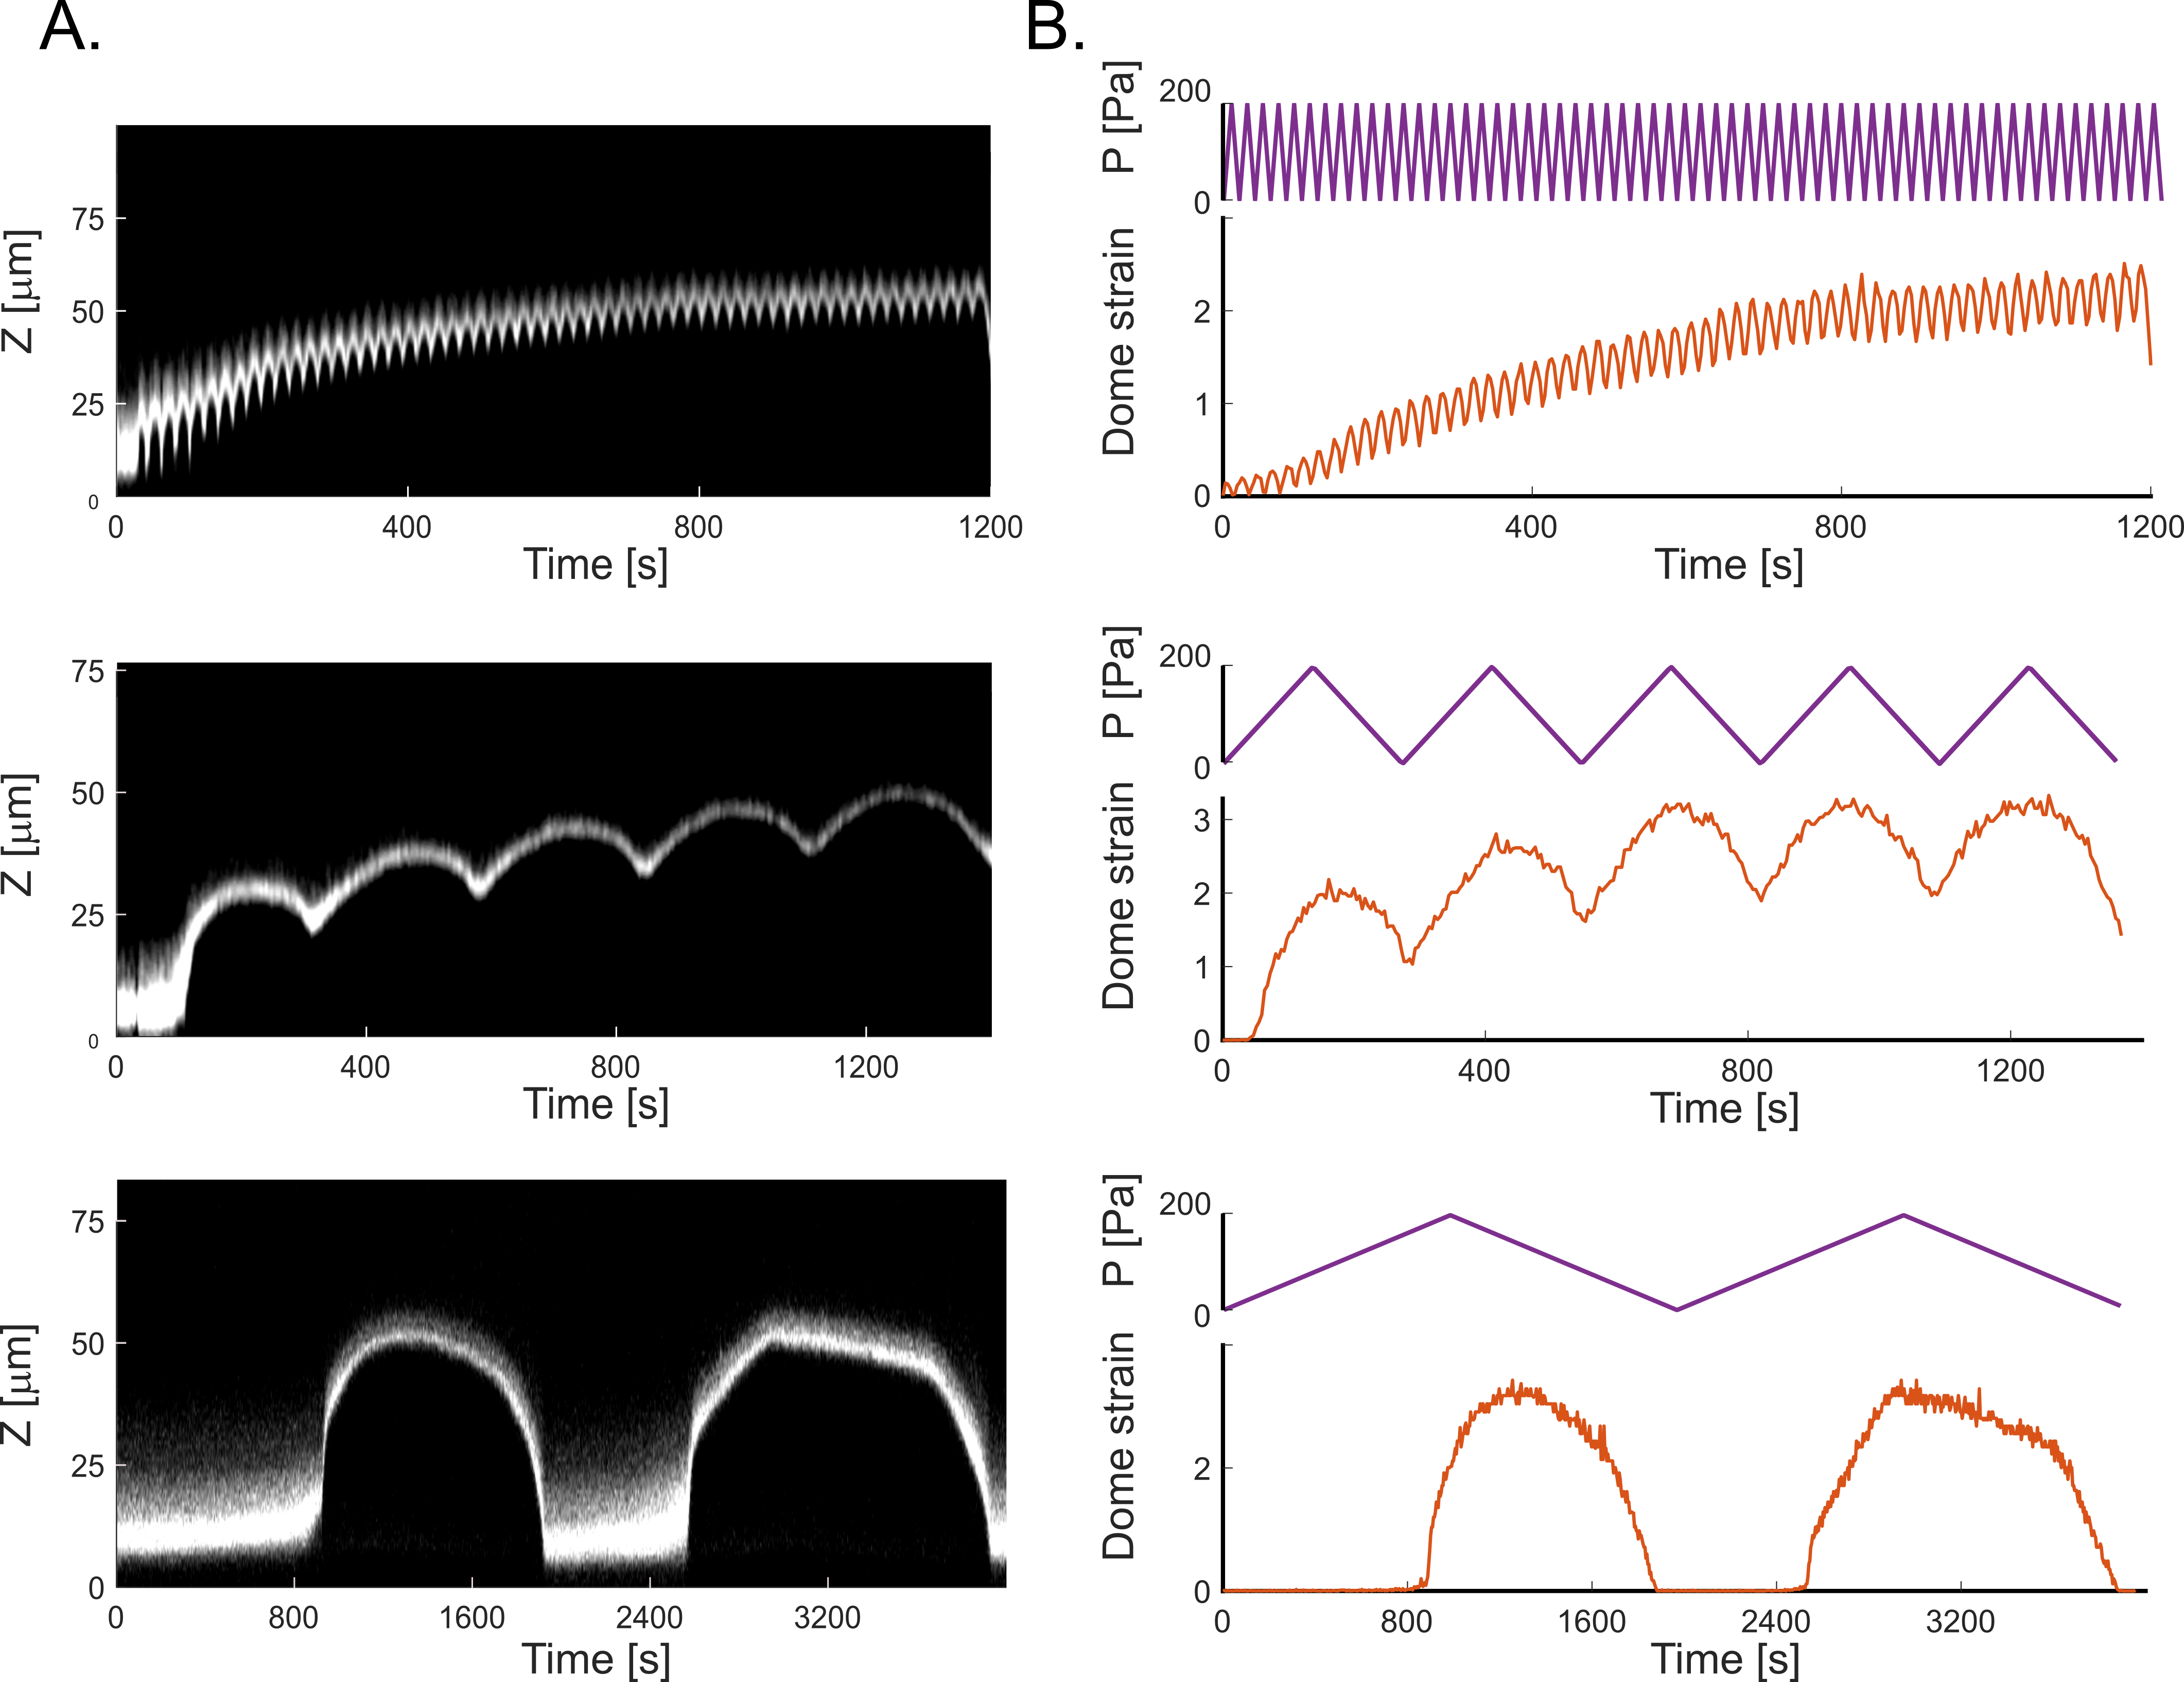
\includegraphics[width=\textwidth]{chap7_dynamic.png}
	\caption{\label{fig_7_6} \textbf{Dynamic response of Epithelia:} (A) The XZ plane images and kymographs of domes subjected to cyclic pressure between 0 to 200 Pa with rates of 20, 1.5, and 0.2 Pa/s The kymographs generated along the midsection of the domes indicated by yellow dotted lines. These indicate the evolution of height of the domes with respect to time. (B) The strain response of domes to cyclic pressure with different rates. Magenta represents pressure and red represents strain with respect to time. For A, B, n= 7 domes for 20 Pa/s, n = 8 for 1.5 Pa/s, and n = 7 for 0.2 Pa/s. 
	}
\end{figure}

In the slowest loading experiments, consisting of two cycles of 2000s, we observed that the domes did not form at lower pressures. As discussed earlier, the domes remained attached until a pressure of 100-150 Pa was attained, beyond which they underwent rapid inflation, leading to high strains of 200-350\%. A clear phase-shift was visible between pressure and strain. In contrast with the previous two cases, the second cycle did not reach a higher strain as compared to the first one (see Fig.~\ref{fig_7_6} B bottom). In these experiments, cells were able to stretch four times their original area and return to the original size at the end of each cycle.

These experiments clearly demonstrated the rate-dependent response of the domes, with faster rates resulting in lower strains and progressive strain accumulation and slower rates allowing for reversibly large deformations. Several features such the remanent strain after a cycle, its ratcheting behavior, the existence of limit cycles, or the phase-shift are suggestive of a viscoelastic material response. We further examine this response next with the help of a computational model.

%\cite{PhysRevLett.94.098103} % optical stretcher
%\cite{Fischer-Friedrich:2016aa} % escachar
%\cite{doi:10.1098/rsos.190920} %unified
%\cite{PULLARKAT200729} % ott review
%\cite{Fernandez_2007} % shear of monolayer
%\cite{clement2017} % One junction
%\cite{khalilgharibi2019} % monolayer stretch


%\newpage

\hypertarget{active-gel-tissue-model}{%
	\section{Active gel tissue model}\label{active-gel-tissue-model}}


Viscoelasticity has been invoked to interpret mechanical measurements of cells and tissues in a variety of contexts, and experimental setups \cite{PULLARKAT200729}, including individual cell-cell junctions \cite{clement2017}, single cells \cite{PhysRevLett.94.098103,Fischer-Friedrich:2016aa}, or cell monolayers \cite{Fernandez_2007,khalilgharibi2019}. In all these examples, experimental curves such as those in Figure \ref{fig_7_6} are fitted by variants of phenomenological rheological models, which may include the short-time power-law rheology measured at cellular and tissue scales   \cite{PULLARKAT200729,doi:10.1098/rsos.190920,khalilgharibi2019}. However, because MOLI allows us to simultaneously measure tissue rheology and image dome and cellular shape in 3D, we sought to pair this device with a computational model that more realistically describes epithelial domes as compared to the common 1D rheological models. Furthermore, the connection between the mechanics of cell monolayers and the structure and dynamics of sub-cellular load-bearing structures, such as the actin or the intermediate filament cytoskeletons is increasingly understood \cite{latorre2018,khalilgharibi2019,duque2023}. These proteins and their dynamics can be visualized and perturbed pharmacologically or optogenetically within MOLI.

For these reasons, we established a close collaboration between the author of the present thesis and Adam Ouzeri, simultaneously developing a theoretical and computational thesis. The main idea of the model is summarized next, and we refer to Adam Ouzeri's forthcoming thesis in the same doctoral program for further details. The model geometrically describes the tissue as a collection of individual cells in 3D defined by triangulations of their bounding surfaces, very much like a vertex model with curved faces \cite{alt2017,perez-gonzalez2021}. However, rather than describing the mechanics of the system using surface tensions, springs or dashpots, it aims to connect tissue mechanics and sub-cellular cytoskeletal dynamics, Figure~\ref{fig_7_2}~A. 

\begin{figure}
	\centering
	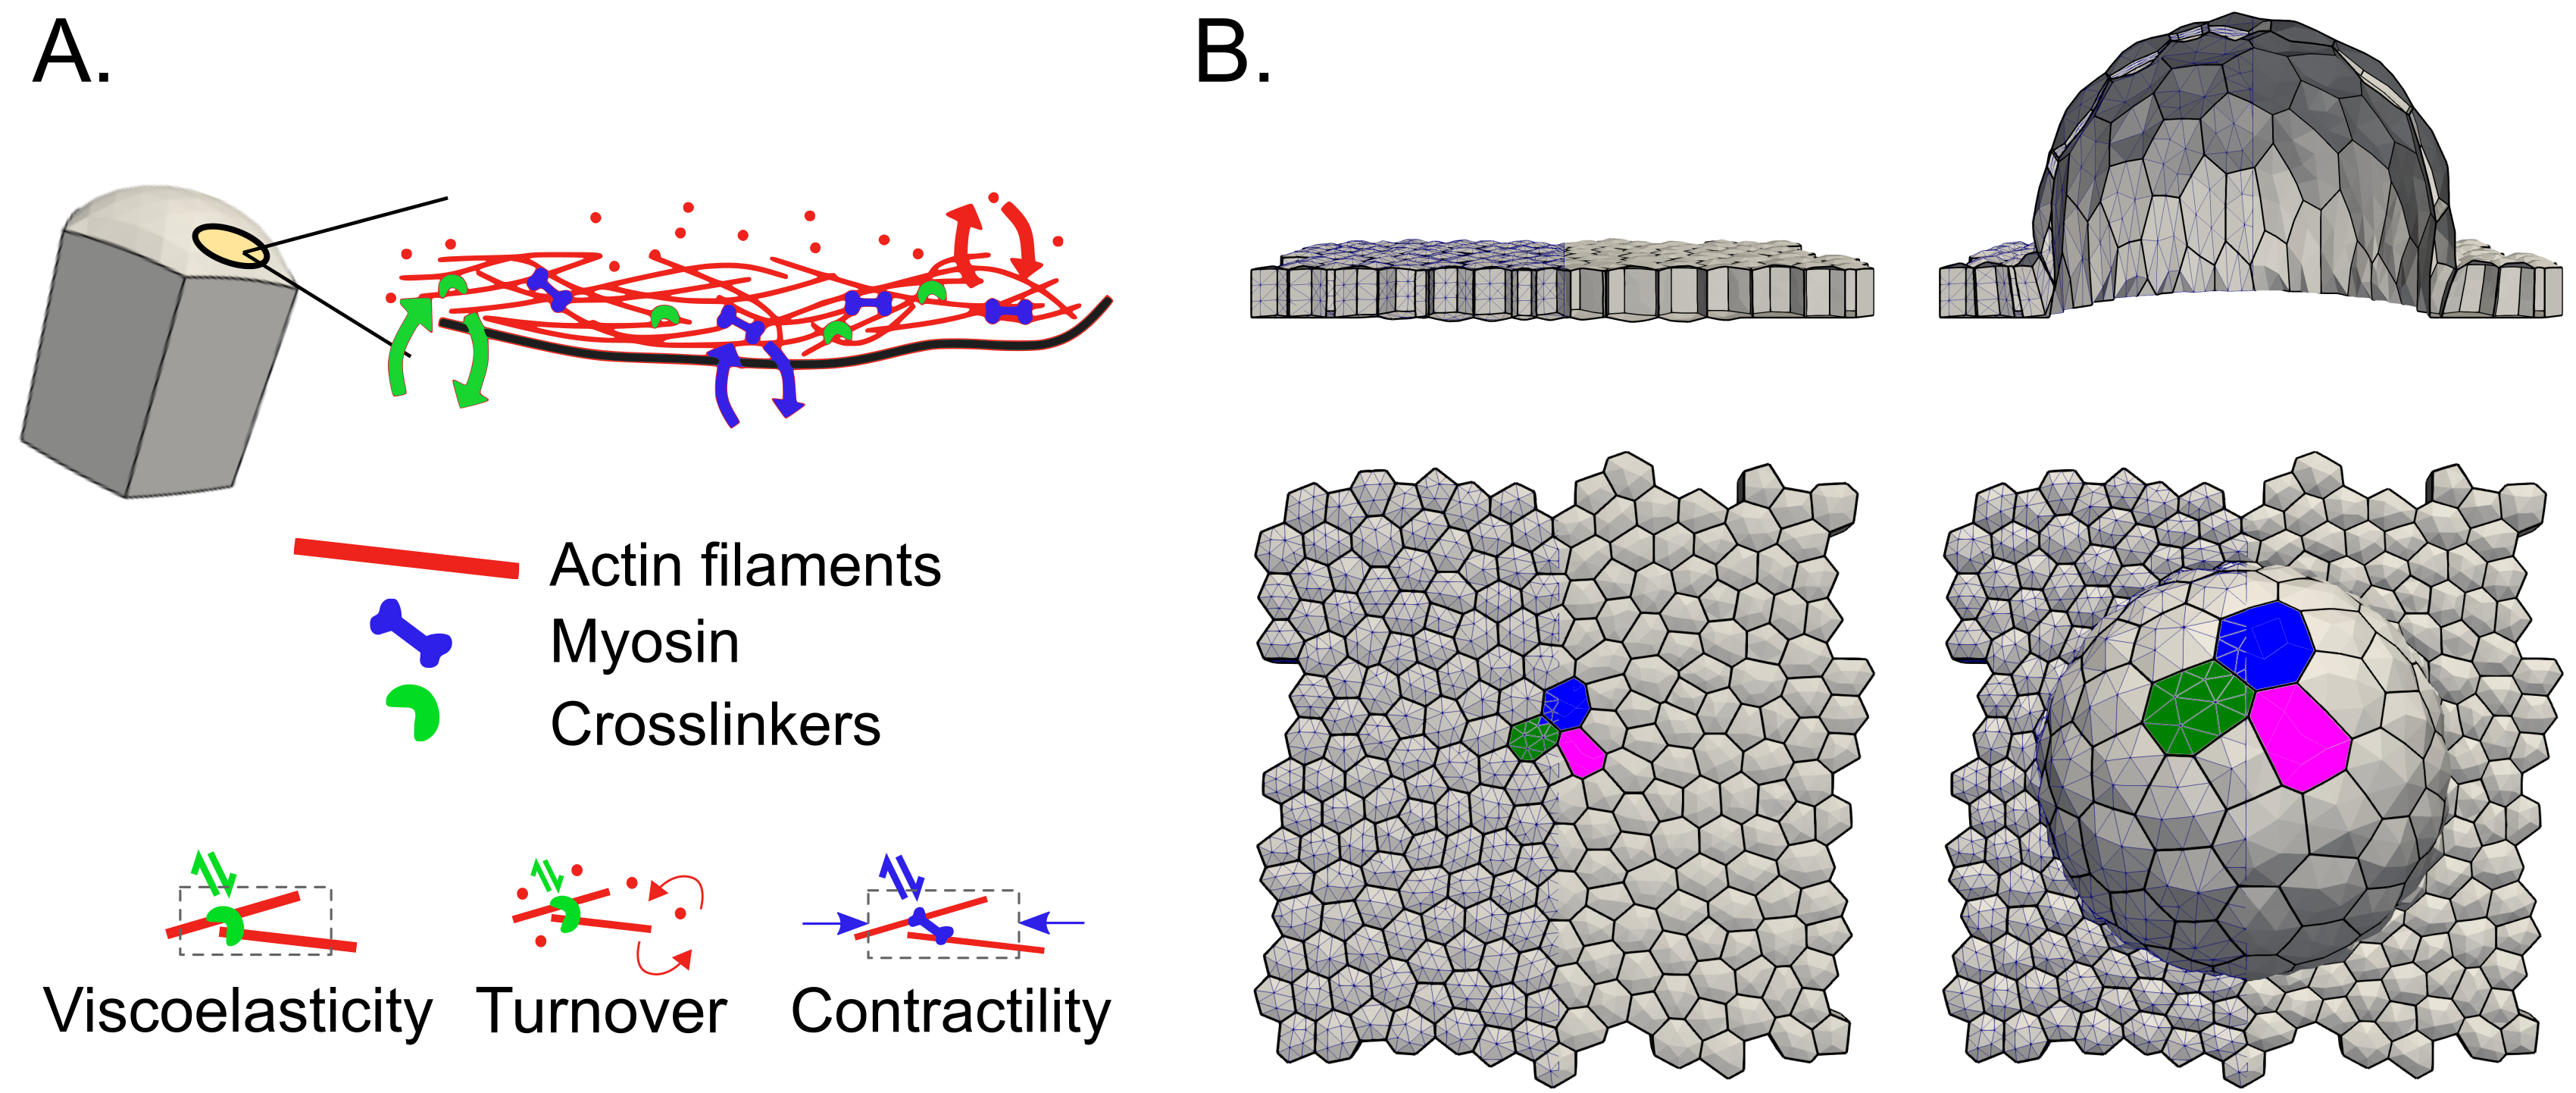
\includegraphics[width=\textwidth]{chap7_digitaldome.png}
	\caption{\label{fig_7_2} \textbf{Active gel tissue model}: (A) The cell is modeled as an active gel of cortex, which mainly comprises three aspects: viscoelasticity of the network, turnover dynamics, and active contractility. (B) These cells can be assembled into a tissue that can be used to perform in-silico experiments. An example of this is the digital dome being inflated, color is highlighting individual cells increasing their area.}
\end{figure}


Focusing on the cortical actin cytoskeleton as a major determinant of epithelial mechanics \cite{latorre2018,khalilgharibi2019,duque2023}, we describe this active interface using the framework of active gel theory \cite{Prost:2015aa}. Active gels provide a coarse-grained continuum description of the actin cortex. In a minimal active gel model of the actin cortex, stresses in the gel have a viscous component capturing the stress relaxation as transient crosslinkers turnover, and an active and density-dependent component capturing contractility due to myosin motors. Cortical materials are advected by the flow, and also polymerize and depolymerize. These models can be enriched to account for multiple cytoskeletal components, for the signaling networks that control their behavior, for their nematic or polar architecture, or for the elastic stresses supported at short time-scales. These models have successfully explained a number of biological behaviors including amoeboid motion of single cells \cite{callan2013} or the formation of supracellular actin patterns \cite{hannezo2015}, and can be improved by comparison with controlled experiments and with agent-based discrete simulations \cite{cortes2020}. 

The tissue model considered here describes each cellular surface in the cell monolayer as an active gel interface. Cell volume is kept constant. The modeling framework can be systematically improved by including other mechanical modules of epithelial cells and their interactions, such as cell-volume regulation, intermediate filaments, cell-cell adhesions, the nucleus, or the plasma membrane. Here, in addition to the active gel surfaces, we include an unspecific mechanical barrier to excessive cellular stretch or compression that becomes active at large strains to capture the tissue strain-stiffening in tension, e.g.~due to intermediate filaments \cite{latorre2018,duque2023}, and the expected stiffening in compression due to nuclear resistance.

The active gel model used here describes the cortex in terms of its shape and of its thickness or cortical areal density \(\rho\), governed by a mass conservation equation accounting for advection, polymerization and depolymerization, which maintains a cortical thickness at steady-state. When deformed rapidly, the crosslinked actin filament network behaves like an elastic network of semi-flexible filaments, which we describe with a hyperelastic model characterized by Lamé parameters  (\(\lambda,\mu\)). Consequently, upon deformation, it can store elastic energy at short timescales. At longer timescales, the network dynamically reorganizes, dissipating the stored elastic energy and relaxing elastic stresses. For instance, the unbinding of a crosslinker in a deformed network will release elastic energy into the frictional environment and re-bind in a partially relaxed network. The dissipation of elastic stresses is represented by viscosity coefficient \(\eta\). Mathematically, the model keeps track of the metric tensor as a multidimensional generalization of the resting length of the network, which evolves over time driven by elastic stresses. The contractile active tension in the network \(\gamma\) is hypothesized to be isotropic and  proportional to cortical thickness as $\gamma(\rho) = \xi \rho$, with proportionality constant  \(\xi\). 

Hence, in a steady-state, cortical density is uniform, elastic and viscous stresses vanish, and we are left with uniform surface tensions as in a conventional vertex model. Out-of-equilibrium, the dynamics of the tissue, and in particular its shape and mechanical behavior, are then direct consequences of the active gel surface dynamics assembled into a monolayer of cells with constant volume, Figure \ref{fig_7_2}. In particular, three timescales emerge from the theoretical framework: 
\begin{enumerate}
	\item Turnover timescale \(t_{to} = 1/k_{d}\)
	\item Viscoelastic timescale \(t_{ve} = \eta/\lambda\)
	\item Viscoactive timescale \(t_{va} = \eta/\xi\)
\end{enumerate}

The turnover timescale is given by the depolymerization rate \(k_{d}\). The viscoelastic timescale is a ratio of the viscous remodeling coefficient to the Lamé parameters, representing elasticity. Lastly, the viscoactive timescale is the ratio of the viscous remodeling coefficient to the coefficient of active tension. For instance, at time-scales smaller than $t_{to}$, cortical stretching or compression leads to deformation-induced changes in cortical thickness, which dissipate over time because of turnover. Likewise, at time-scales smaller than $t_{ve}$, the cortex behaves like an elastic interface whereas at times much larger than $t_{ve}$ it flows like a viscous fluid. 

Using this model, a virtual representation of a cell monolayer can be generated with specific boundary conditions. In particular, we can create a cell monolayer with regions that lack basal attachment to the substrate, which can be inflated into domes under pressure application, similar to the experimental setup, Figure \ref{fig_7_2} B. These simulations will be referred to as "digital domes" in subsequent discussions. By employing this model and comparing the results with the experimental data, we can effectively understand and investigate the biomechanical properties of epithelial tissues, specifically the contribution of the viscoelasticity of the actin cortex.


\hypertarget{active-viscoelasticity-of-the-epithelia}{%
	\section{Active viscoelasticity of the
		epithelia}\label{active-viscoelasticity-of-the-epithelia}}
	
In this section, we interpret the experimental results within the context of the active gel tissue model. %The mathematical framework describes how cells, represented as an active gel, change shape. Specifically, the initial shape, known as the reference configuration (\(\Gamma_{0}\)), is mapped to its current shape, called the deformed configuration (\(\Gamma\)). This mapping enables the quantification of strains and deformations relative to the reference configuration using a metric tensor, which measures distances and angles within the material. When a material is deformed, the distances and angles within it change, and the metric tensor reflects these changes. In this case, each configuration possesses its own metric tensor.
%For typical elastic materials, the reference configuration remains fixed in time, and deformations are measured relative to this fixed state. However, to account for the remodeling of the cortex through dynamic crosslinking, our model considers the reference configuration as dynamic, necessitating a time-varying metric tensor  (\(\mathbf{G}\)). We can refer to this evolving reference configuration as the resting frame. By employing the dynamic metric tensor, we can calculate the resting area of a cell, which represents an imagined area where all stored elastic energy is dissipated. In terms of cell area, the relationship between the resting area (\(A_{rest}\)) and the actual area (\(A_{actual}\)) can be expressed as
%\begin{equation}
%	A_{rest} = \int_{\Gamma_0} \sqrt{|\mathbf{G}|}dS_0, \text{ and } A_{actual} = \int_{\Gamma}dS.
%\end{equation}
%Where $dS_{0}$ and $dS$ are infinitesimal area on the cortex in reference and deformed configuration respectively.
%In the case of a polymer with dynamic crosslinks, the resting area of the material changes as the crosslinks break and reform in response to applied stress. The updated resting area can be used as a dynamic reference configuration for measuring subsequent deformations of the material.
Consider an example where the tissue is step stretched biaxially. The actual area of apical and basal faces  changes instantly, and becomes larger than the resting length. Consistent with volume conservation, lateral faces also change in area, and also in shape. Hence the cortex as an elastic network stores recoverable strain energy. However, as cross-links and filaments turnover, this energy dissipates. In the model, the metric tensor evolves over time in such a way that the resting area (and shape for lateral surfaces) progressively becomes equal to the actual area (shape), thus relaxing over time the elastic stresses (see Fig. \ref{fig_7_7a} A). We call this time-dependent stresses associated with the relaxation of the metric tensor viscoelastic. On top of these stresses, the cortex sustains active stresses, which are also time-dependent because they are proportional to cortical density, and the step stretch instantly dilutes apical and basal faces and concentrates lateral faces, which then recover the steady-state thickness due to turnover. The net effect of such active viscoelastic behavior of individual faces on the tension of a tissue made of identical cells is shown in  Figure~\ref{fig_7_7a}~B. This figure depicts the stress relaxation dynamics of the tissue.

\begin{figure}[b!]
	\centering
	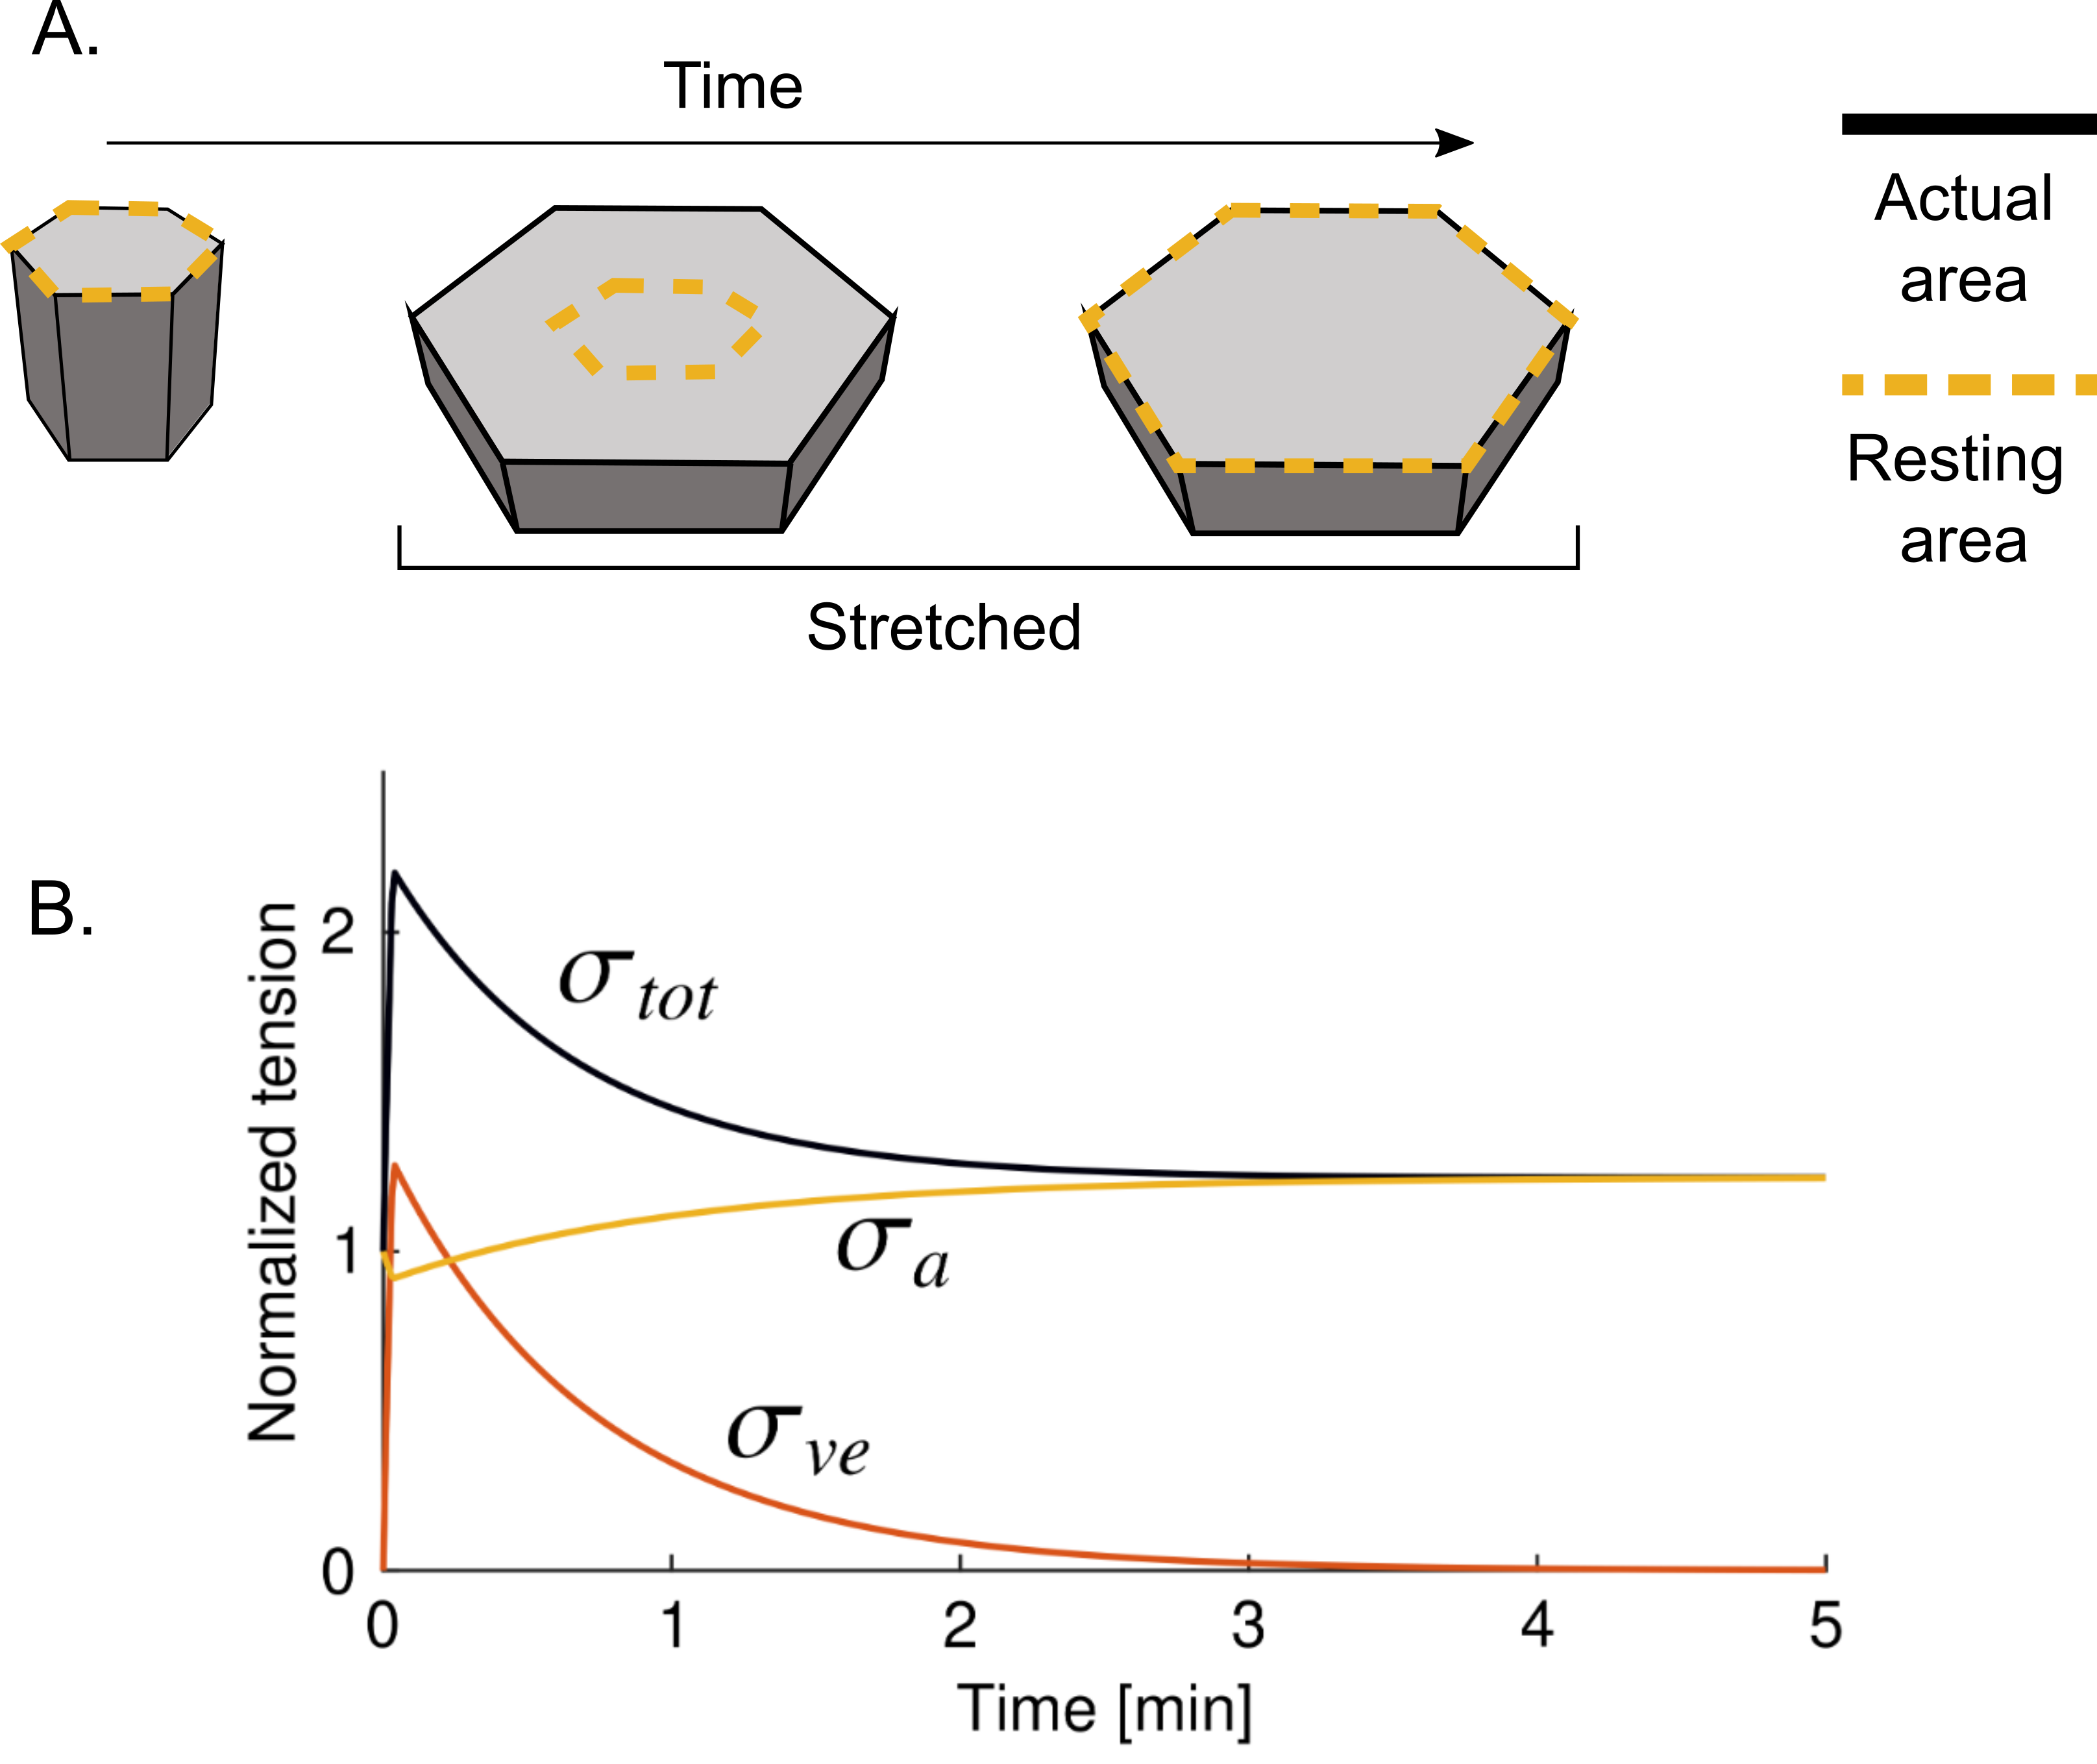
\includegraphics[width=0.8\textwidth]{chap7_area1.png}
	\caption{\label{fig_7_7a} \textbf{Active viscoelastic response after step deformation}: (A) Illustration of a resting and actual area of a cell in a tissue during stretching. (B) Evolution of total tissue tension (black), viscoelastic stress (red), and active tension (yellow) in response to step deformation.
	}
\end{figure}

However, as discussed earlier, MOLI does not naturally probe a strain-controlled mechanical ensemble. Thus,  simulations were conducted to mirror the experimental conditions. Upon subjecting the digital dome to constant pressure, consistent with our previous experimental observations, the digital dome reached a steady state strain while experiencing a reduction in tissue thickness as the cells stretched, Figures \ref{fig_7_7} A and \ref{fig_7_2} B. The remodeling of the cortex dissipates the viscoelastic stress and increases the active tension. At steady state, only the active tension remains balancing the externally applied pressure. The simulations show that the time to reach the steady state is mainly driven by the viscoelastic timescales. During such dynamics, the digital domes also produced the  non-monotonous tension-strain relations observed experimentally, Figure \ref{fig_7_7} B.

To map the steady-state constitutive relation, we first quasi-statically increased pressure to obtain the blue curve in Figure \ref{fig_7_7} B. We then  mirrored the experimental procedure by subjecting the digital domes to pressure steps, and then letting the system reach a steady state. We found that these tension-strain pairs at steady state for different pressures retrace the blue quasi-static curve in Figure \ref{fig_7_7} B. This curve displays characteristics similar to those observed experimentally. The strain-stiffening at high strains can be attributed to the barrier mechanism introduced to limit high strains, which we did not attempt to fit to experimental measurements. 


\begin{figure}[]
	\centering
	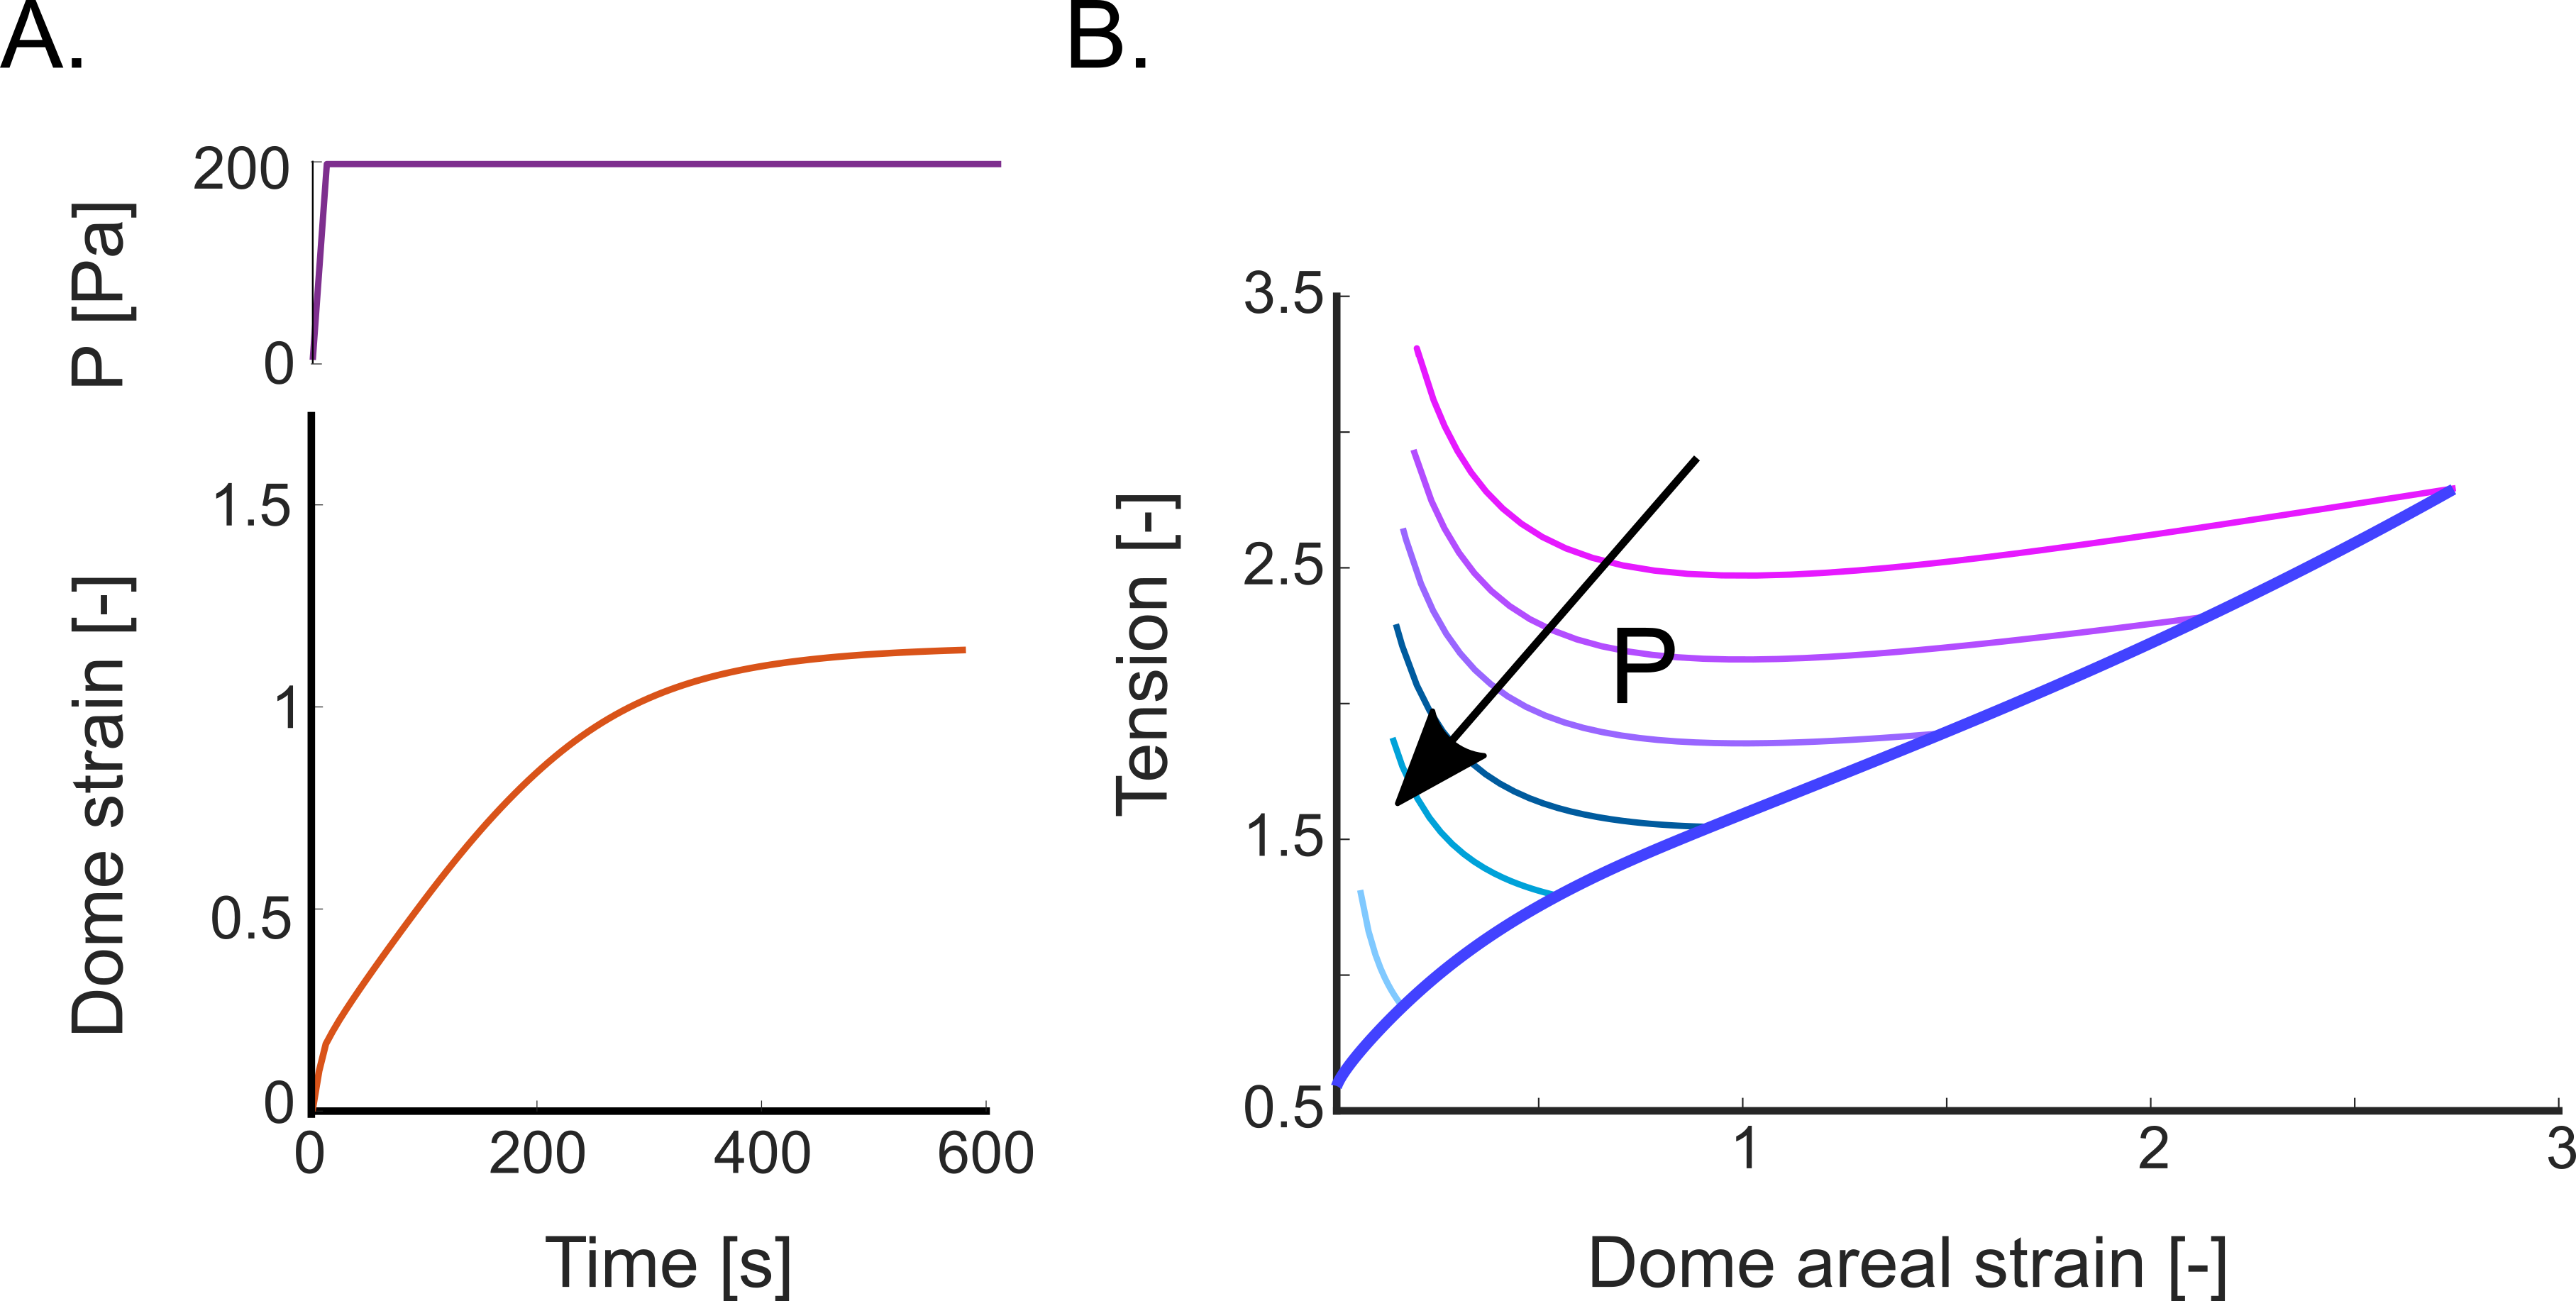
\includegraphics[width=\textwidth]{chap7_constitutivelawtwin.png}
	\caption{\label{fig_7_7} \textbf{Material response of the digital domes}: (A) When subjected to constant pressure, as in experiments, the digital dome inflated and reached a steady state. (B) These simulations also produced non-monotonic tension strain curves for different pressures, all leading to a steady state. The blue curve is the result of a quasi-static increase of pressure, which traces the locus of steady-state points obtained in long isobaric simulations. Tension reported here is non dimensional.}
\end{figure}

The effect of the remodeling timescale is particularly noticeable in cyclic stretching experiments. When digital domes are subjected to a cyclic pressure at rates that are slower than cortical dynamics, then the cortex remains close to steady state during cellular deformations. Hence, the stored elastic energy is rapidly dissipated as the strain increases, and the cortical thickness does not change significantly as turnover has time to restore the steady-state thickness. We observed that the resting area in the digital dome almost overlapped with the actual area (see Fig.~\ref{fig_7_8} B bottom). This slow rate of 0.2 Pa/s provides cells with sufficient time to remodel and dissipate viscoelastic stresses. Viscoelastic and turnover timescales in simulations are around 10-30s, which means that over a period of 2000s, the dome stretches to considerably large strains of 250-300\% and returns to its original flat state.


\begin{figure}
	\centering
	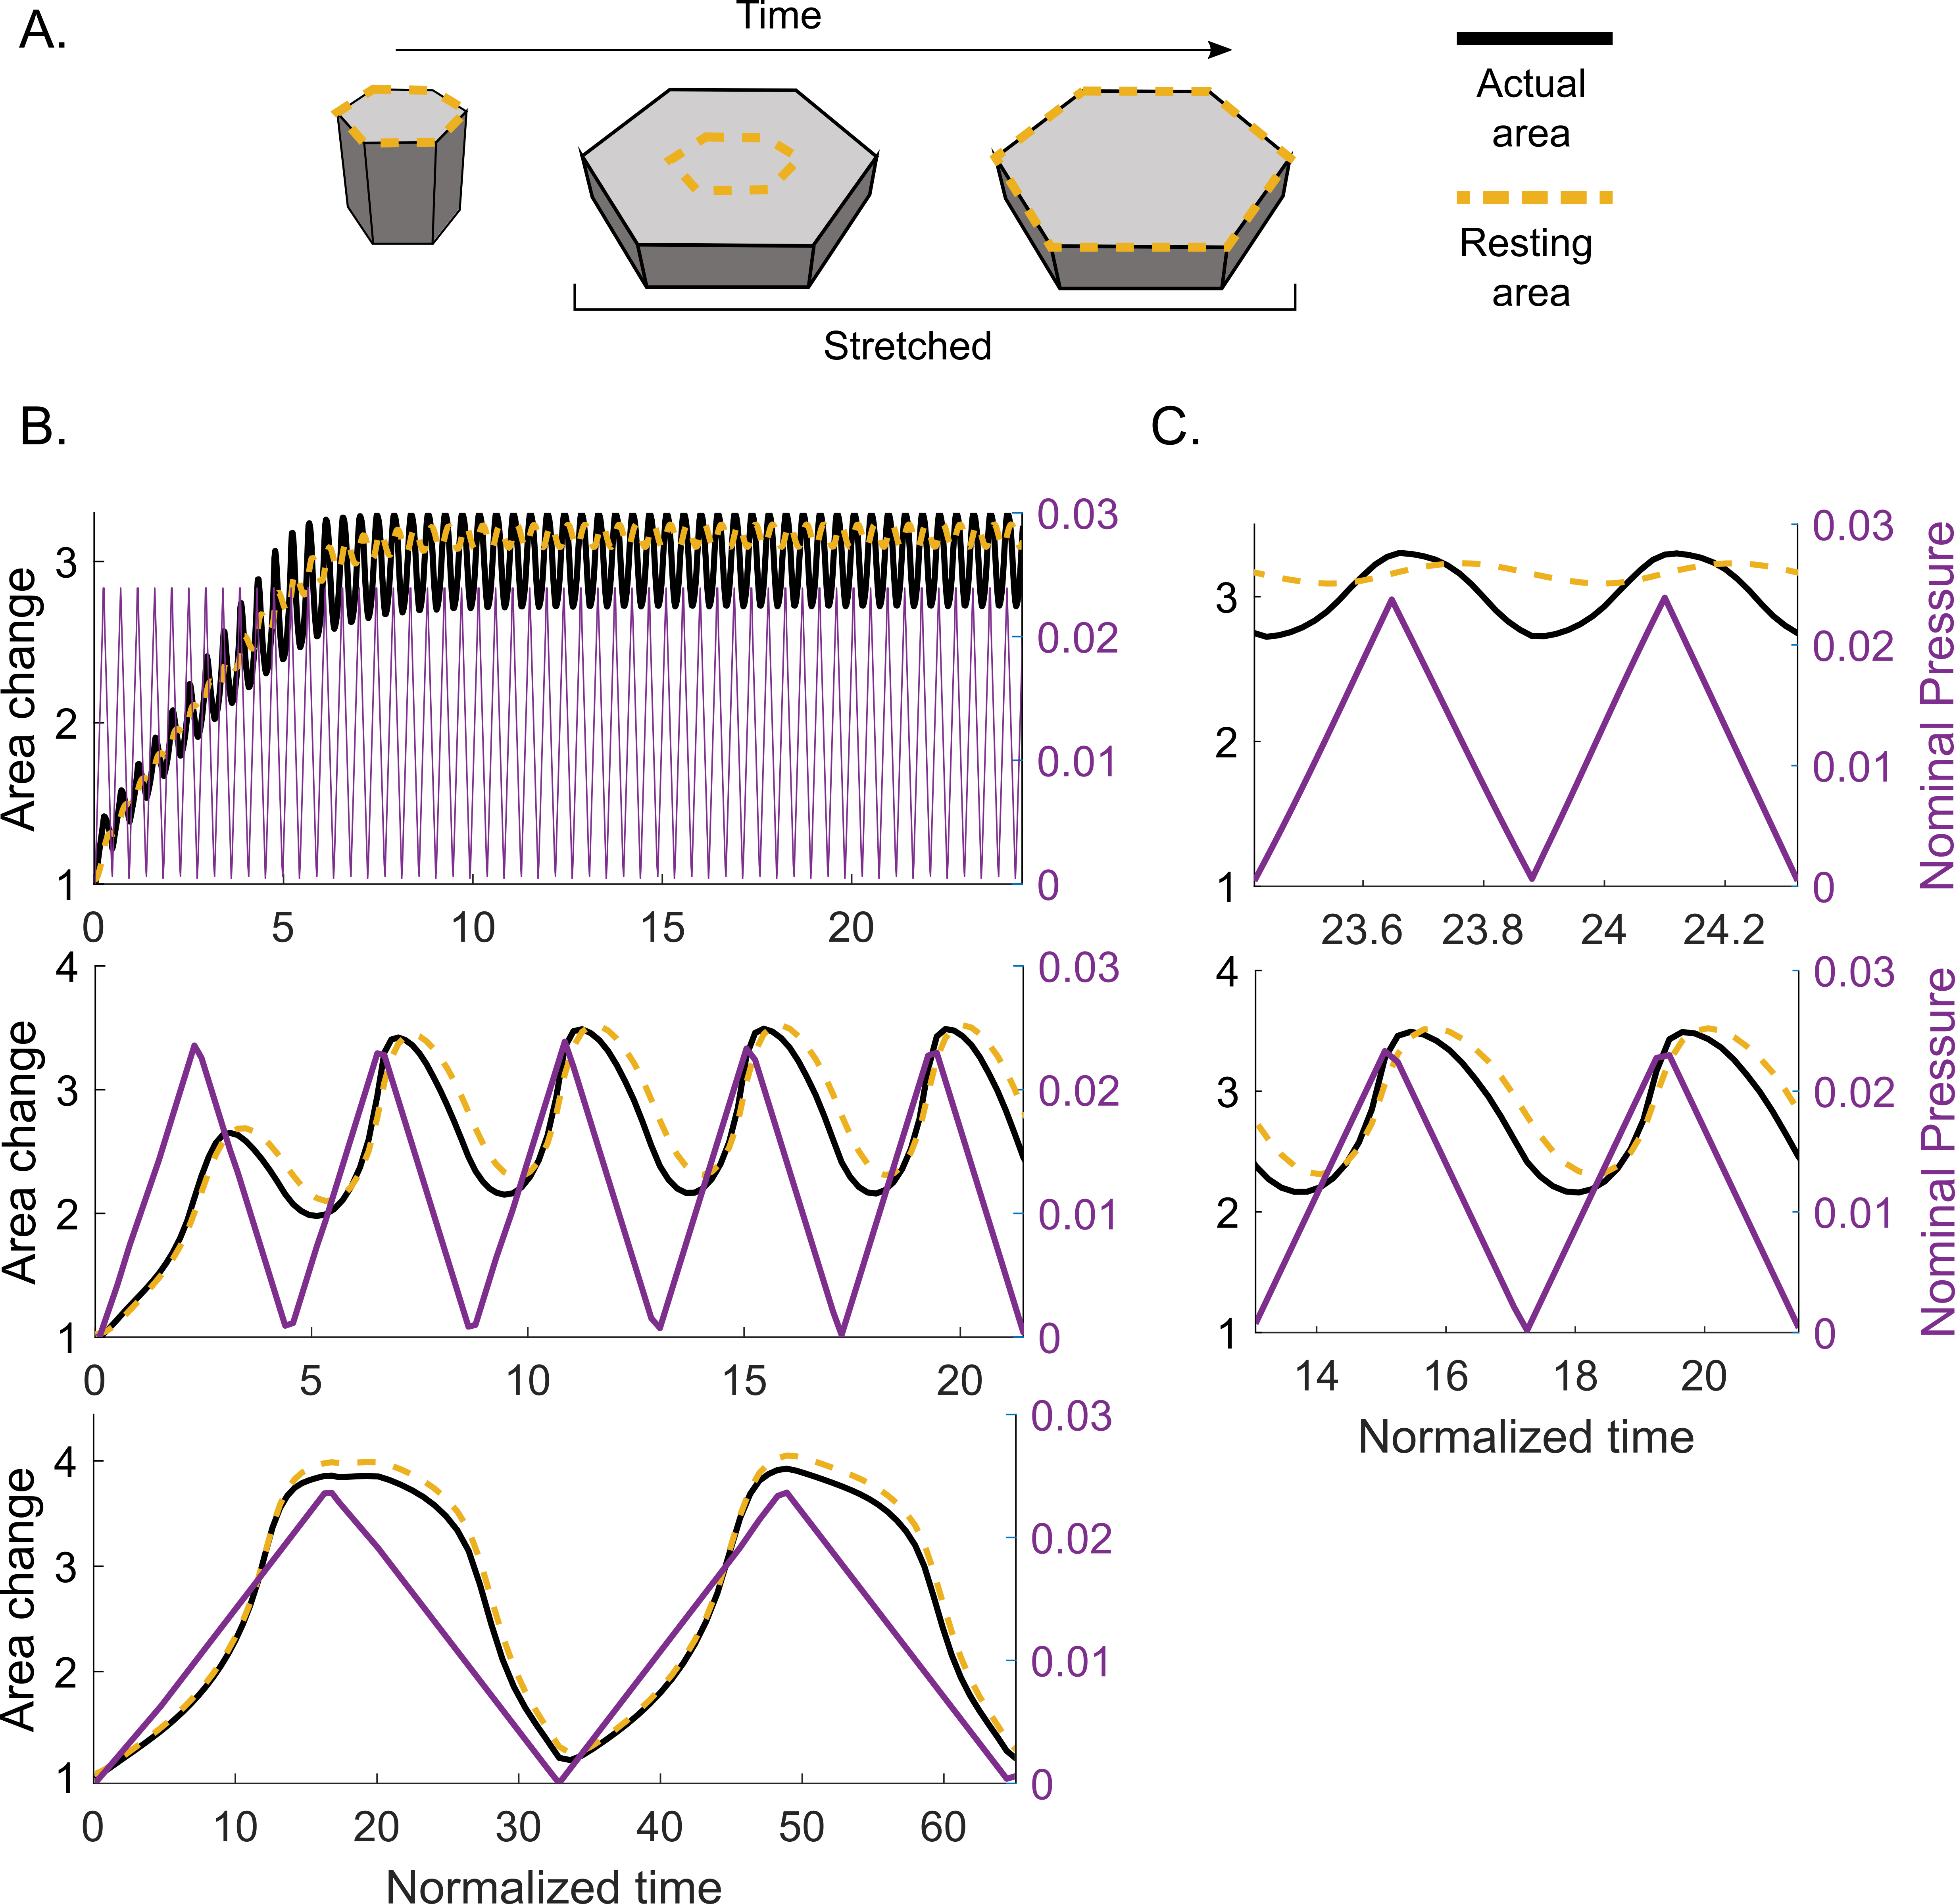
\includegraphics[width=\textwidth]{chap7_area.png}
	\caption{\label{fig_7_8} \textbf{Evolution of Resting and Actual Cell Areas in Response to Cyclic Pressure}: (A) Illustration of resting and actual cell areas in a monolayer during stretching. (B) Fold area change relative to the initial area, with three rows of panels showing the evolution of area change over normalized time. Digital domes were subjected to cycles with three different time intervals: 20s (top), 266s (middle), and 2000s (bottom). (C) Inset of the last two cycles in the case of fast and moderate rates.
	}
\end{figure}


In contrast, when cells in a dome are subjected to cyclic pressure at rates faster than cortical dynamics, they accumulate strains due to insufficient time to dissipate viscoelastic stress. In this case, the actual area changes more rapidly than the viscoelastic and turnover timescales permit (see Fig.~\ref{fig_7_8} B top). Consequently, along with the change in the actual area, the resting area also changes, but at a slower pace. During deflation, the resting area decreases but cannot decrease completely before the next inflation cycle begins, causing the tissue to stretch further in a ratcheting behavior reported in individual cell junctions \cite{clement2017}. Eventually, a limit cycle is reached, wherein cells stably oscillate between two strains, and the resting area oscillates as well, but at a smaller amplitude (see Fig.~\ref{fig_7_8} B top).

To sum up, the active gel model explains the material response of epithelial tissue depending on the rate at which pressure is applied. The concept of resting area enables us to interpret that slower rates allow for cell remodeling and dissipation of viscoelastic stress, while faster rates result in strain accumulation due to insufficient time for dissipation. This active viscoelastic behavior is the outcome of timescales associated with cortical remodeling.


\hypertarget{summary}{%
	\section{Summary and Discussion}\label{summary}}

In this chapter, we investigated the mechanics of epithelial tissue by applying pressure at varying rates. Initially, we applied a constant pressure of 200Pa, which led to the dynamic inflation of domes eventually reaching a steady state in strain. Due to the spherical geometry of the tissue and Laplace’s law, we observed a non-monotonous tension-strain curve in response to the constant pressure. We identified such curves as an intrinsic feature of the isobaric mechanical ensemble with fixed footprint area, natural with MOLI. This understanding allowed us to trace steady-state tension strain curves from the steady-states at different pressures, and found constitutive relations with increasing tension with respect to strains at lower values, but appearing to plateau at higher strains. 

Furthermore, our measurements showed that the domes accumulated strain through the cycles when probed with fast-changing pressure and reached a limit cycle in later cycles. However, when stretched slowly, the domes reached higher strains without accumulating strain at the end of the cycle. To understand the behavior of epithelial tissue, we used a modeling and computational framework, which explains the tissue mechanical response from the active viscoelasticity of the cell cortex \cite{ouzeri2023}. The digital dome studies highlighted the interplay of different timescales, which are the reflection of the interaction between cortical turnover, crosslinker dynamics, and network reorganization. 

%Our results can be interpreted using a multidimensional Maxwell model. The classical Maxwell model consists of a spring and a dashpot, which represent the elastic and viscous elements, respectively. In our case, we can imagine a similar model with two branches: one branch includes a spring and a dashpot to represent the passive viscoelasticity, and a second branch includes an active spring to represent the active component  (see fig \ref{fig_7_9}). The active spring is always present, but if the system is stretched at slower rates, the dashpot drives the dominant mechanical response. Conversely, if stretched at faster rates, the elastic spring deformation dominates. By separating the passive and active components, we can better understand how each contributes to the overall viscoelastic behavior and associated timescales. 

%\begin{figure}[b!]
%	\centering
%	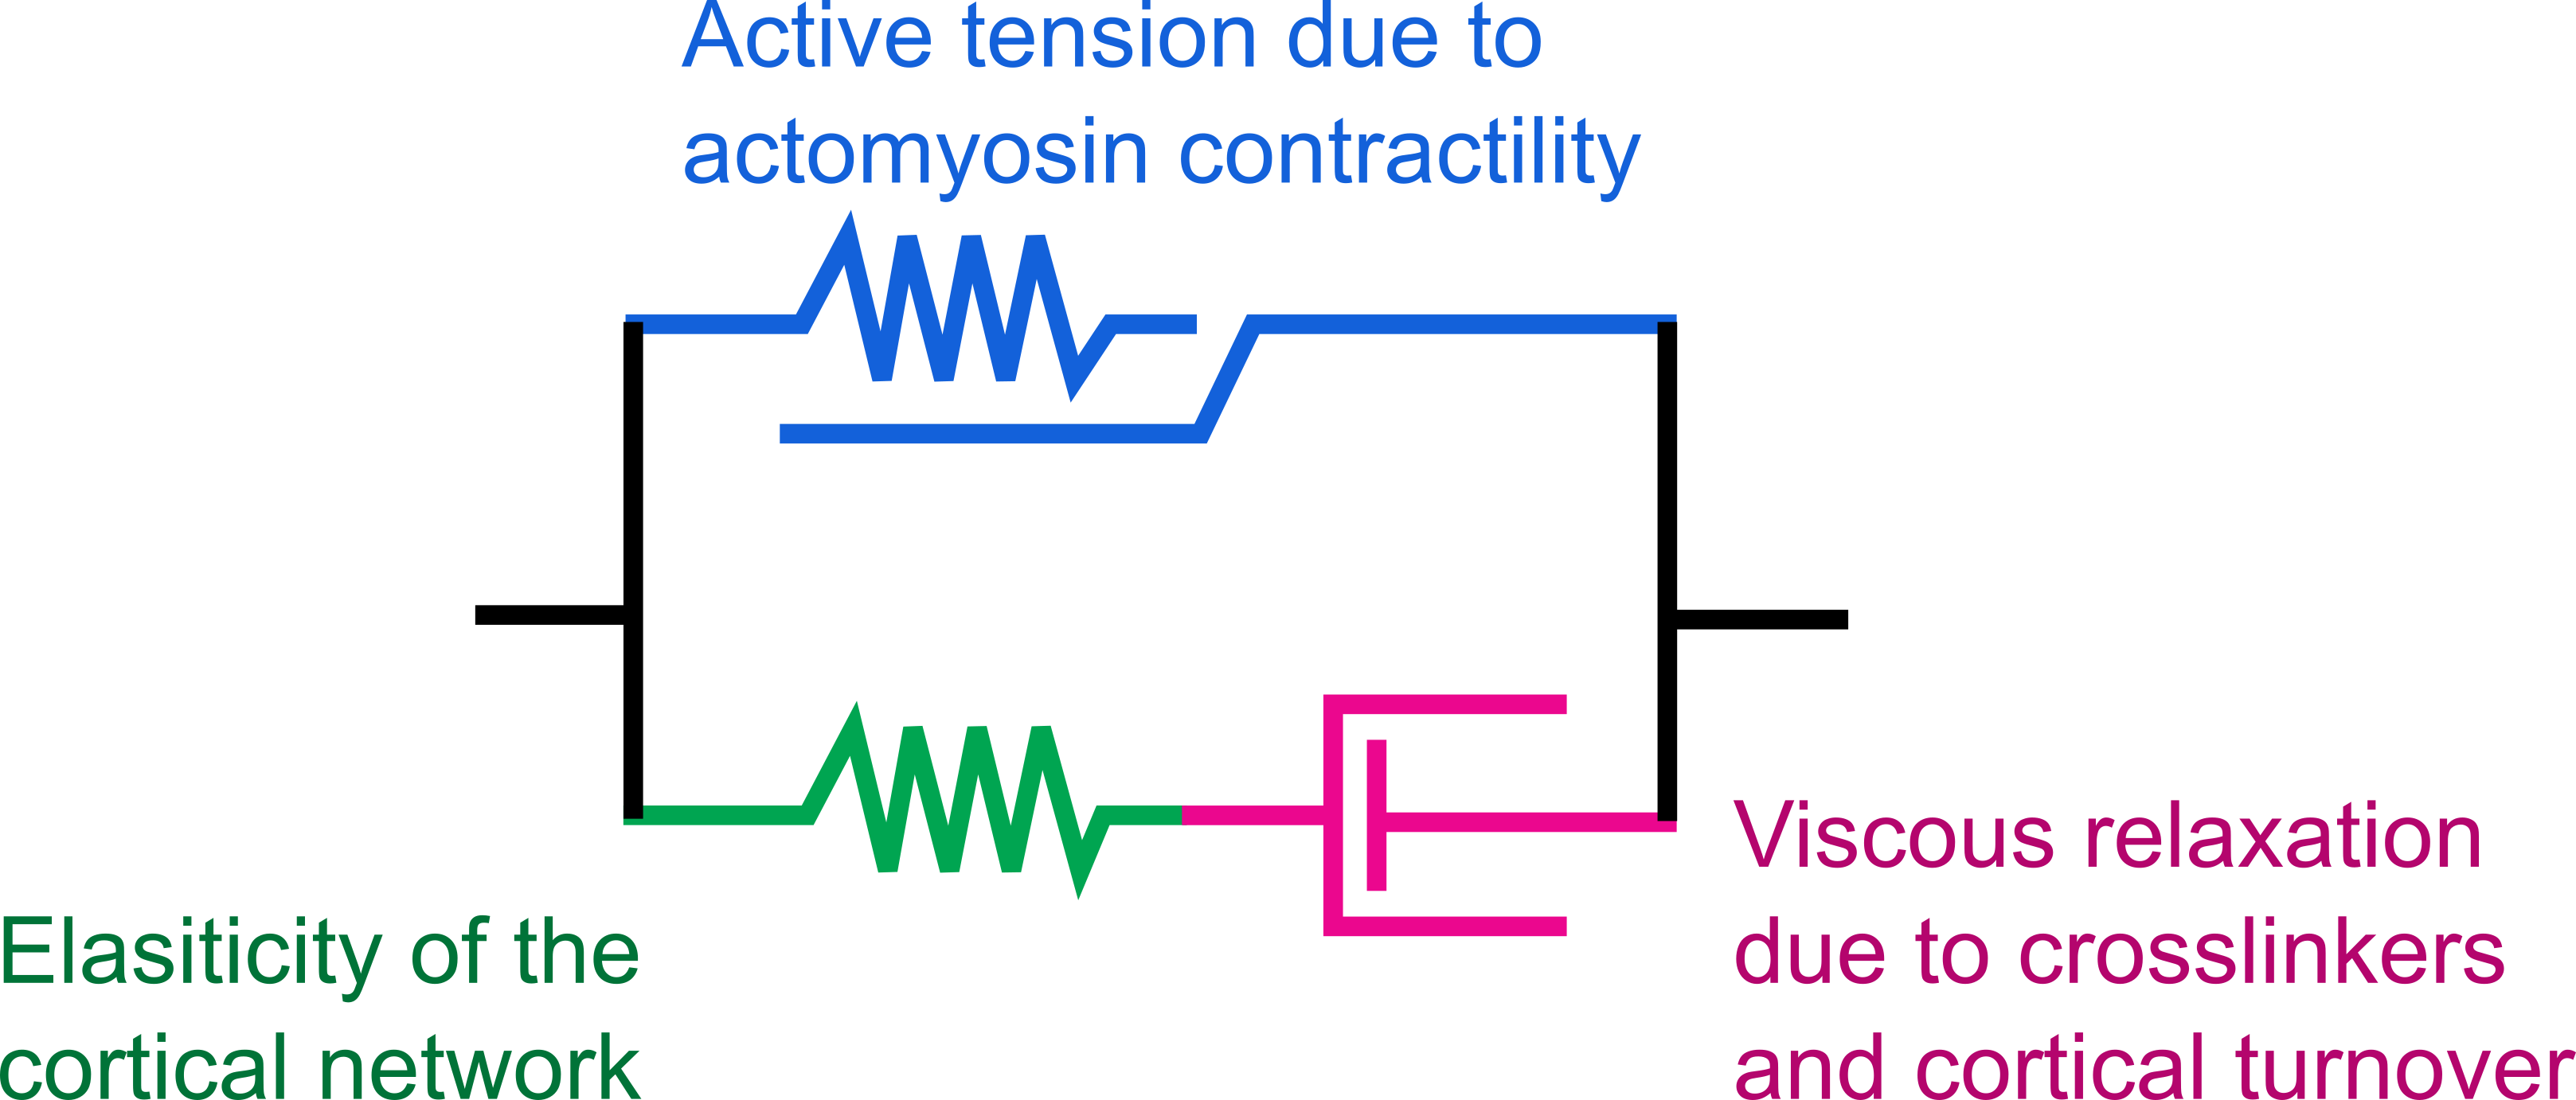
\includegraphics[width=0.75\textwidth]{chap7_maxwell.png}
%	\caption{\label{fig_7_9} \textbf{Representational viscoelasticity model}: The model can be understood using a spring and dashpot analogy with two branches: The first branch is an active spring representing the contractile forces applied by the actomyosin cortex. The second branch has two components, one for the elasticity of the network and the second for the viscous relaxation that occurs due to turnover of the network.
%	}
%\end{figure}

Previous research has approached the viscoelastic rheology of cell monolayers using minimal rheological models involving springs and dashpots. One particularly interesting model was developed by \citet{khalilgharibi2019}, which characterizes the response of a suspended monolayer to stretch and demonstrates that the dynamics are similar to that of a single cell, due to the role of the actomyosin cortex. They used a model with two springs in parallel, one of which can change its resting length dynamically. The model explains the relaxation of the monolayer, as the active contractility of the cortex changes the resting length of the active spring, which closely relates to our "resting area" concept. 

Another study by \citet{clement2017} found that viscoelastic dissipation could explain the shortening or elongation of cell junctions in Drosophila embryos. They demonstrated that the dissipation occurs at the minute timescale, which coincides with myosin pulses, and that actin turnover plays a key role in this dissipation. These pulses have a ratchet-like mechanical effect that drives junction shortening and causes tissue folding. This ratcheting effect is reminiscent of the cyclic stretching at faster rates, where cells stretch more and more every cycle. Similar to the authors of the study, we explain the strain accumulation by incomplete dissipation of viscoelastic stress due to deformation faster than the remodeling timescale.
The multi-cellular model used here recovers these phenomenologies and relates them to cytoskeletal dynamics. More importantly, it is applicable to more general situations in which the cellular deformation are heterogeneous, as further discussed in the next chapter. 

Regarding molecular components, although we did not use pharmacological treatments, the MOLI system can accommodate the introduction of drugs. Various components in the actin network enable cortical tension modulation through pharmacological interventions that target specific molecular targets \cite{cartagena-rivera2016}. For instance, Latrunculin depolymerizes the actin network, while Blebbistatin decreases cortical tension by inhibiting myosin activity. Conversely, Calyculin-A enhances contractility by accelerating Myosin II phosphorylation. In future experiments, these pharmacological interventions could be used to identify the molecular pathways involved in the tissue's mechanical response.

Our experimental system focused on probing the response of suspended tissues at short timescales (minutes), which correspond to the timescale of actomyosin network remodeling. We did not observe any cellular rearrangement, extrusion, or division at this timescale in our system, except for rare exceptions. Long-term experiments were not performed, as they were outside the scope of this study due to the suspected involvement of other cytoskeletal components, such as intermediate filaments. \citet{latorre2018} observed the activation of intermediate filaments in extremely stretched cells (>300\%) and proposed that this reorganization caused restiffening, preventing  cells from stretching excessively. This observation motivated the strain-limiting mechanism imposed in our model.

\citet{latorre2018}  also demonstrated heterogeneity in cell stretching, attributed to a mechanism of  active superelasticity. However, in our experiments, we did not observe the coexistence of stretched and super-stretched cells. This might be due to the relatively shorter timescales in our experiments compared to long-term and pulsating deformation of spontaneous domes.

A recently published study \cite{duque2023} shows that strain stiffening at very large strains is dependent on the strain and strain rates. The tissue stiffens at higher strains, but for higher strain rates, the stiffening is more pronounced. % at higher strains (15\%) than lower strains (120\%). [remove this because I a not sure it is correct, and this paper uses linear strains whereas you use areal strains] Nimesh's reply: TRUE 
They demonstrated that this response is due to the supracellular network of intermediate filaments. Because in MOLI we do not control strain directly but rather pressure, it is not straightforward to map our results and those in this study. However, it is possible in principle to control strain and strain rate by a feedback mechanism. %\marino{[I am not sure if this is what you mean.]}  NImesh's reply: I almost meant this, I thought we could quantify the strain rates in the cyclic stretching experiments but feedback mechanism is better.
%In our experiments, we could only control pressure and pressure rates. However, if needed, we can track the strains and quantify strain rates to explore the mechanics. 
% When plotting tension-strain curves for different pressure rates, we noticed characteristics of stiffening at higher strains and higher rates \marino{[this is not shown, I am not sure it the reader will understand]}. 
We further note that in the model, we did not include any rate-dependence in the strain stiffening as proposed by \citet{duque2023}, but it can be easily incorporated as mechanistic and quantitative understanding of this process becomes available.


Having established the correspondence of our computational model and experiments in MOLI, which depicts  the epithelium as an active viscoelastic material, we will harness in the next chapter this understanding to control dome shape transformations.
